\chapter{Evaluation of Existing Frameworks} \label{cha:evaluation}

In order to determine a viable GPU implementation strategy for the physical core of ASUCA it has been necessary to analyse the available industry standards and whether they are already suited for JMA's needs as is (see also sec.~\ref{sub:thesisMotivation}). 

Sec.~\ref{sec:criteriaPortation} lists the evaluation criteria. In sec.~\ref{sec:investigatedFrameworks} the investigated GPGPU software frameworks are being introduced. The CPU compilers used for comparison are listed in sec.~\ref{sec:investigatedCPUCompilers}. Sec.~\ref{sec:testHardware} introduces a performance model for the test hardware. Sec.~\ref{sec:testCases} lists the test cases used for the evaluation. Sec.~\ref{sec:usabilityComparison} compares the frameworks in terms of usability while sec.~\ref{sec:perfEvaluation} compares the frameworks by performance. Sec.~\ref{sec:evalConclusion} draws a preliminary conclusion about the viability and performance of the tested frameworks for the purpose of an ASUCA physical process implementation.

\section{Criteria for an ASUCA Physical Process GPU Portation} \label{sec:criteriaPortation}

The following criteria are important to consider when choosing a framework for the GPGPU portation of the ASUCA physical process codebase: 

\begin{enumerate}
 \item \label{crit:fortranGPU} The framework should offer a GPGPU interface for a Fortran 90 codebase.
 \item \label{crit:hybrid} The framework should make a hybrid codebase possible, i.e. the user code should be compilable to both GPU and CPU. This allows the verification of results on the CPU before porting, testing and debugging the GPU implementation.
 \item \label{crit:smallChanges} Required code changes to the existing codebase should be as small as possible in order to lower the portation cost.
 \item \label{crit:performance} It should offer viable execution time performance, i.e. it should be as close to fully platform optimized code as possible. If possible, the performance should be viable both on CPU and GPU. This would give two additional advantages:
  \begin{enumerate}
    \item The modules could be ported one-by-one and integrated into the current production environment, allowing for a smoother transition and easier validation.
    \item Heterogenous execution would become an option at a later point, such that the code would become portable to a wide range of clusters / supercomputers.
  \end{enumerate}
 \item \label{crit:agnostic} It should be as platform and software vendor agnostic as possible, e.g. Open Source frameworks and industry standards are preferred.
\end{enumerate}

\clearpage
\section{Investigated GPU Frameworks and Compilers} \label{sec:investigatedFrameworks}

The frameworks presented in this section have been evaluated with respect to the criteria stated in sec.~\ref{sec:criteriaPortation}. 

\subsection{OpenACC} \label{sub:openACC}

For an introduction to CUDA please refer to sec.~\ref{sub:openACCIntro}. For the implementation criterias stated in sec.~\ref{sec:criteriaPortation}, OpenACC is the solution the most promoted by the industry right now. Though it must be noted that currently, no compiler completely supports the OpenACC 1.0 standard. The support has been improved over the course of this thesis, however. It is also promising, that MeteoSwiss, responsible for the Swiss weather prediction model in association with the European Consortium for Small Scale Modelling (COSMO), is also involved in an OpenACC portation project for their physical processes. Lst.~\ref{listing:absswOpenACC} in cha.~\ref{cha:analysis} shows a sample OpenACC implementation.

For this evaluation the following OpenACC capable compilers have been tested: 

\begin{enumerate}
 \item PGI Workstation (\verb|pgcc| and \verb|pgf90|), version 12.4
 \item CAPS HMPP, version 3.1.0
\end{enumerate}

Both compilers offer C as well as Fortran frontends for OpenACC. PGI compilers have been executed with the following flags when used for OpenACC compilation, if not stated otherwise: 

\begin{description}
 \item[-acc] Enables OpenACC compilation.
 \item[-ta=nvidia,cc20] Specifies the target platform, in this case NVIDIA GPUs with computing capabilities version 2.0.
 \item[-O4] The highest optimization level for PGI compilers.
\end{description}

The HMPP framework is essentially a preprocessor that creates CUDA kernels for parsed OpenACC directives and passes the host code to an underlying compiler of the user's choice. For fair comparison, \verb|pgcc| was chosen as the underlying compiler using the same settings as presented above.

\subsection{CUDA C} \label{sub:cudaC}

CUDA C is NVIDIA's proprietary C language extension. For an introduction to CUDA, please refer to sec.~\ref{sub:cudaIntro}. As an implementation strategy for the ASUCA physical process it is not viable, since it violates the criterias \ref{crit:fortranGPU} and \ref{crit:smallChanges} stated in sec.~\ref{sec:criteriaPortation}. However, it was used as a performance validation, since CUDA C implementations can generally be optimized the closest to GPUs from NVIDIA, other than writing PTX device instructions.

For this thesis we have tested NVIDIA's CUDA framework in version 4.1. 

CUDA C requires a third party C compiler for host code compilation. For the tests discussed in this chapter, \verb|pgcc| has been used with the following compiler flags:

\begin{description}
 \item[-Mcuda=cc20] Enables CUDA compilation for 2.0 CUDA device architecture.
 \item[-O4] The highest optimization level for PGI compilers.
\end{description}

\subsection{PGI CUDA Fortran} \label{sub:cudaFortran}

PGI CUDA Fortran is a Fortran 90 wrapper framework developed and maintained by The Portland Group. It creates CUDA C code from Fortran kernel and device function definitions. The CUDA C version is then compiled using a NVIDIA CUDA compiler. In that regard, CUDA Fortran can be expected to perform on the same level as CUDA C for a given feature set - however the implemented features tend to lag behind those released by NVIDIA, such as support for \verb|printf| in kernels as well as device code debugging. 

PGI CUDA Fortran, like CUDA C, would require deep restructuring of the ASUCA Physical Process codebase, however it has been used in order to compare the usability and performance to OpenACC implementations. 

Again, PGI Workstation version 12.4 has been used for testing the CUDA Fortran framework. The following compiler flags have been used for \verb|pgf90| when compiling for CUDA Fortran:

\begin{description}
 \item[-Mcuda=cc20] Enables CUDA Fortran compilation for 2.0 CUDA device architecture.
 \item[-O4] The highest optimization level for PGI compilers.
 \item[-Minline=levels:5,reshape] Enables inlining for routines defined in the same module as their caller. The \verb|reshape| option enables the compiler to perform array reshaping when passing them to the callee.
\end{description}


% \subsection{Other Available Technologies} \label{sec:otherTechnologies}
% 
% Listed here for completeness
% 
% \begin{description}
%  \item[OpenCL] Open Computing Language (OpenCL) is a nonproprietary standard for hybrid computational programming maintained by the Khronos Group~\cite{OpenCL}. Its role is very similar to that of CUDA, with its main advantage being the portability of code to GPUs of manufacturers other than NVIDIA (i.e. AMD and Intel). For the scope of this project it was however decided to not further investigate the use of OpenCL, since its available Fortran interfaces were not considered mature enough. Please note however, that the proposed solution presented in the chapters \ref{cha:framework} and \ref{cha:implementation} makes an OpenCL implementation possible at a later point without changing the user code. 
% \end{description}

\clearpage
\section{Investigated CPU Compilers} \label{sec:investigatedCPUCompilers}

The version 11.1 of Intel C (\verb|icc|) and Intel Fortran (\verb|ifort|) compilers have been used for reference purposes throughout this thesis. 

% \begin{description}
%  \item[Intel C and Intel Fortran] in version 11.1, specifically \verb|icc| and \verb|ifort|.
%  \item[PGI Workstation] in version 12.4, specifically \verb|pgcc| and \verb|pgf90|.
% \end{description}

Various experiences have shown that this compiler offers the most consistant optimizations (without the need to adjust and experiment with various tuning screws) when used on the vendor provided hardware. For this reason the Intel compilers appear to be a reasonable choice for the determination of the CPU performance reference on Intel hardware. \verb|icc| and \verb|ifort| have been used with the following compiler flags, if not stated otherwise: 

\begin{description}
 \item [-fast] Enables the compiler to use the optimization settings leading to the highest performance based on its internal heuristics. This includes vectorization and inlining of routines as well as enabling the \verb|-O3| arithmetic optimization level.
\end{description}

\clearpage
\section{Hardware Model} \label{sec:testHardware}
Since the scope of this thesis has been to implement and analyse single GPU as well as single CPU performance, only one CPU socket and one GPU has been used for the performance analyses in sec~\ref{sec:perfEvaluation} as well as chapter \ref{cha:analysis}. This section gives an overview over the hardware performance model used for performance estimates throughout this thesis.

\subsection{Overview FP Performance and Memory Bandwidth} \label{sub:hardwarePerfOverview}

For all tests, single Tsubame 2.0 nodes have been used in the following configuration~\cite[p. 4]{TSUBAMEUserGuide}: 
\begin{enumerate}
 \item One Dual socket Intel Xeon X5670 CPU with 6 cores per socket. One Xeon X5670 socket offers the following performance metrics~\footnote{Theoretical CPU performance is based on the assessment for X5650 in~\cite[p. 4]{LatticeBoltzmannMulticoreCPU}, with the computational performance numbers scaled by $2.93 \unit{GHz}\diagup 2.66 \unit{GHz}$ in order to adjust for the Xeon X5670's higher frequency~\cite{XeonX5670Specs}.}:
  \begin{enumerate}
    \item 1 Core Sustained Memory Bandwidth\footnote{Single core stream memory bandwidth is based on~\cite[p. 7]{ArithmeticsOnWestmere}.}: \verb|9.8 GB/s|
    \item 1 Socket Sustained Memory Bandwidth: \verb|20.5 GB/s|
    \item 1 Core Single Precision Peak Performance: \verb|23.4 GFLOPS|
    \item 1 Core Double Precision Peak Performance: \verb|11.7 GFLOPS|
    \item 1 Socket (6 Core) Single Precision Peak Performance: \verb|140.1 GFLOPS|
    \item 1 Socket (6 Core) Double Precision Peak Performance: \verb|70.1 GFLOPS|
  \end{enumerate}
 \item Three NVIDIA Tesla M2050 GPUs. One Tesla M2050 offers the following performance metrics~\cite{TeslaC2050Specs}:
  \begin{enumerate}
    \item Sustained Memory Bandwidth\footnote{The Tesla M2050's sustained Memory bandwidth has been evaluated using the bandwidth test program provided in the CUDA SDK.}: \verb|108.4 GB/s|
    \item Single Precision Peak Performance: \verb|1030 GFLOPS|
    \item Double Precision Peak Performance: \verb|515 GFLOPS|
  \end{enumerate}
\end{enumerate}

It is important to note that the peak computational performance usually does not directly translate into sustained performance, however it is reasonable to take the relative ratios into consideration: One might expect a Tesla M2050 to enable the following speedups:
\begin{description}
 \item[11.1 times] faster for memory bandwidth bounded algorithms compared to single core CPU execution.
 \item[5.3 times] faster for memory bandwidth bounded algorithms compared to single socket / six core CPU execution.
 \item[44 times] faster for computationally bounded algorithms compared to single core CPU execution.
 \item[7.4 times] faster for computationally bounded algorithms compared to single socket / six core CPU execution.
\end{description}

However there are many architectural differences that have not been taken into consideration for this line of thought. For this reason it is necessary to do tests with the actual programs in order to make reasonably well founded performance predictions. 

\subsection{System Balance} \label{sub:hardwareSystemBalance}

For further discussions the notion of \textquotedblleft System Balance\textquotedblright\ will be defined as follows: 

\textit{System Balance is the number of floating point instructions per floating point fetch or store, that leads to a maximum floating point throughput while utilizing the maximum sustained memory bandwidth.}

That is, system balance is defined using the following formula\footnote{This notion of System Balance is based on the Roofline model by Patterson~\cite{Roofline}. Patterson uses the notion of ``operations per byte'' as an indicator for boundedness. The test hardware used for this thesis offers double precision peak performance exactly half of single precision peak performance, both for CPU and GPU - therefore the memory bandwidth is being adjusted by the length of the floating point values such that the balance estimate can be used both for single and double precision execution.}:

\begin{equation}
    \text{System Balance} = {\text{Peak FLOPS} \over {\text{Sustained Memory Throughput}\over\text{Size of Floating Point Variables}}}
\end{equation}

One issue to keep in mind when taking into account peak \verb|GFLOPS| numbers: Vendors calculate these by doubling the effective throughput of floating point operations per cycle, assuming a program would only generate \verb|multiply-add| instructions (which can be scheduled in one cycle by modern high performance architectures). Assuming that effectively \verb|10%| of the instructions are \verb|multiply-add|, one gets a more reasonable prediction of fp performance using the following calculation:
\begin{equation}
  \text{Peak FLOPS} = {\text{Peak FLOPS}_{\text{vendor}} \cdot (0.1 \cdot 1 + 0.9 \cdot {1 \over 2})} \approx {\text{Peak FLOPS}_{\text{vendor}} \cdot 0.55}
\end{equation}

Considering the metrics introduced in sec.~\ref{sub:hardwarePerfOverview}, the system balances become 
\begin{description}
 \item[5.3] for single core CPU execution (using the following calculation: 
  \begin{equation}
    23.4 \unit{GFLOPS} \cdot 0.55 \over{ 9.8 \unit{GB/s} \over{ 4 \unit{Bytes/FLOP}}}
  \end{equation} 
 ).
 \item[15.0] for six core CPU execution (using the following calculation:
  \begin{equation}
    140.1 \unit{GFLOPS} \cdot 0.55 \over{ 20.5 \unit{GB/s} \over{ 4 \unit{Bytes/FLOP}}}
  \end{equation}
 ).
 \item[20.9] for GPU execution (using the following calculation: 
  \begin{equation}
    1030 \unit{GFLOPS} \cdot 0.55 \over{ 108.4 \unit{GB/s} \over {4 \unit{Bytes/FLOP}}}
  \end{equation}
 ).
\end{description}
These assumptions are valid for both double and single precision since both the computational power and the fetched data per floating point value scale by a factor of two. One must note however, that the above calculations are rather simplistic. One would have to account for many details specific to the architectures, such as operation scheduling, in order to get a more precise performance model - especially in the CPU case, because of its rather intricate architecture, this would be an undertaking not feasible within the scope of this evaluation. 

For qualitative measures it is enough to say that algorithms whose fp instruction to fetch/store ratio is significantly below System Balance, are expected to be bounded by memory bandwidth while algorithms above System Balance are expected to be computationally bounded - the most important distinction to make when trying to optimize for performance. 

\section{Test Cases Used for Comparison} \label{sec:testCases}

As discussed in sec.~\ref{sub:openACC}, OpenACC appears to be the most obvious choice for a portation of the ASUCA physical process. Three modules have been used for evaluating performance and usability of OpenACC: 

\begin{enumerate}
 \item 3D Diffusion
 \item (Single Stage) Particle Push
 \item ASUCA Shortwave Radiation
\end{enumerate}

CUDA C is generally considered to perform the closest to the hardware limit on NVIDIA GPUs since its hardware vendor maintained compiler usually receives new features first. For this reason, CUDA C implementations of the algorithms for \textbf{single stage particle push} as well as \textbf{3D diffusion} have been used in order to determine a baseline performance benchmark for the OpenACC frameworks to compare to.

Since it is easier to compare two C implementations instead of C vs. Fortran implementations, the OpenACC implementations for these two algorithms have been made using the OpenACC C language frontends as well. It is reasonable to assume the results of that comparison in C to be an indicator for Fortran GPU implementations as well, since at least PGI CUDA Fortran and PGI OpenACC use an intermediate CUDA C code representation in order to make use of NVIDIA's \verb|nvcc| compiler.

The \textbf{ASUCA shortwave radiation} module has been used as a benchmark for a real world application, which lead to insights not only for performance but also for the usability of the tested frameworks. The frameworks have been tested in their Fortran incarnations (as described in sec.~\ref{sub:openACC} and sec~\ref{sub:cudaFortran}) for this module since the final goal is a GPGPU implementation of the ASUCA Physical Process using Fortran.

The following subsections offer more details on three test modules introduced above.

\subsection{3D Diffusion} \label{sub:test3DDiffusion}

Lst.~\ref{listing:ppush} shows the 3D diffusion routine used as the first performance benchmark.

This routine is executed with the following specifics:
\begin{itemize}
  \item $256\times256\times256$ data points are being calculated for each timestep. This number has been chosen to be divisible by 32 (to make it best suitable for GPU warps as introduced in sec.~\ref{sec:fermi}) and to result in a long enough execution time such that measuring inaccuracies are not influencing the conclusion.
 \item The input and output pointers are being swapped after every timestep. No data is being copied in between timesteps.
%  \item $0.1 / (1 / 256^2) \approx 6553$ timesteps are being calculated.
 \item $6553$ timesteps are being calculated.
 \item Single as well as double precision arithmetics have been evaluated.
\end{itemize}

A few notes about this algorithm: 
\begin{itemize}
 \item The algorithm is expected to be bounded by memory bandwidth. Disregarding the boundary computations (which only account for ${3\over{3+258}} \approx 1\%$ of calcutions in this configuration) the algorithm leads to seven fetches and one write per $13$ floating point computations, giving a computation-to-fetch ratio of $1.85$, which is clearly in the memory bandwidth bounded region for all metrics displayed in sec.~\ref{sec:testHardware}.
 \item The computation results have been validated against an analytical solution. In case of double precision numerical calculation, the result had a root mean square error of $1.1 \cdot 10^{-6}$, which is expected to be the error of the numerical approximation used here. For single precision calculation, the error was in the order of $10^{-5}$, with slight differences between CPU and GPU execution. (The GPU interestingly calculated with a higher accuracy, $1 \cdot 10^{-5}$ vs. $2 \cdot 10^{-5}$ root mean square error).
\end{itemize}

\begin{lstlisting}[style=cStyle, name=diff3d, label=listing:diff3d, caption={3D Diffusion Example Program.}]

/* ======================
   SETUP OF ONE XY-PLANE
   ======================
  x marks the origin of the coordinate system (beginning of halo)
	   ___________________________________
______x|______haly_______________|pad+halx|
pad+hal|                         |        |
       |                         |        |
       |        dimX * dimY      |        |
       |                         |        |
       |_________________________|________|
_______|______haly_______________| 

*/   

/*
#define ADDR_FROM_XYZ(x, y, z): calculate coordinates in the data
structure shown above, using X-,Y-,Z-dimensions, haloes and paddings
*/

void  diffusion3d_timestep (
   float    *f,    /* dependent variable */
   float    *fn,   /* updated dependent variable */
   int      nx,    /* x-dimensional grid size */
   int      ny,    /* y-dimensional grid size */
   int      nz,    /* z-dimensional grid size */
   float    kappa, /* diffusion coefficient */
   float    dt,    /* time step interval */
   float    dx,    /* grid spacing in the x-direction */
   float    dy,    /* grid spacing in the y-direction */
   float    dz     /* grid spacing in the z-direction */
) {
	
    int    j,  jx,  jy,  jz,  NX = nx + 2,  NY = ny + 2;
    float ce = kappa*dt/(dx*dx), cw = kappa*dt/(dx*dx),
	  cn = kappa*dt/(dy*dy), cs = kappa*dt/(dy*dy),
	  ct = kappa*dt/(dz*dz), cb = kappa*dt/(dz*dz),
	  cc = 1.0 - (ce + cw + cn + cs + ct + cb);
        
    for(jz = 1; jz < nz + 1; jz++) {
      for(jy = 1; jy < ny + 1; jy++) {
        for(jx = 1; jx < nx + 1; jx++) {
          j = ADDR_FROM_XYZ(jx, jy, jz);
          fn[j] = cc*f[j]
          + ce*f[j+1] + cw*f[j-1]
          + cn*f[j+NX] + cs*f[j-NX]
          + ct*f[j+(NX * NY)] + cb*f[j-(NX * NY)];
        }
      }
    }
	    
    // Wall Boundary Condition
    for(jz = 1; jz < nz + 1; jz++) {
      for(jy = 1; jy < ny + 1; jy++) {
        j = (NX * NY)*jz + NX*jy + 0;
        fn[j] = fn[j+1];
        j = (NX * NY)*jz + NX*jy + nx + 1;
        fn[j] = fn[j-1];
      }
    }
	
    for(jz = 1; jz < nz + 1; jz++) {
      for(jx = 1; jx < nx + 1; jx++) {
        j = (NX * NY)*jz + NX*0 + jx;
        fn[j] = fn[j+NX];
        j = (NX * NY)*jz + NX*(ny + 1) + jx;
        fn[j] = fn[j-NX];
      }
    }

    for(jy = 1; jy < ny + 1; jy++) {
      for(jx = 1; jx < nx + 1; jx++) {
        j = (NX * NY)*0 + NX*jy + jx;
        fn[j] = fn[j+(NX * NY)];
        j = (NX * NY)*(nz + 1) + NX*jy + jx;
        fn[j] = fn[j-(NX * NY)];
      }
    }
}
\end{lstlisting}


\subsection{Particle Push} \label{sub:testParticlePush}

Lst.~\ref{listing:ppush} shows the very simple particle push timestep routine used as the second performance benchmark.

This routine is executed with the following specifics:
\begin{itemize}
 \item 6'553'600 ($256 \cdot 256 \cdot 100$) particles are being calculated for each timestep. This number has been chosen to be divisible by 32 (in order to make it best suitable for GPU Warps as introduced in sec.~\ref{sec:fermi}) and to result in a long enough execution time such that measuring inaccuracies can be neglected.
 \item The input and output pointers are being swapped after every timestep. No data is being copied in between timesteps.
 \item 800 timesteps are being calculated.
 \item Single precision arithmetics have been used.
\end{itemize}

Some notes about this algorithm: 
\begin{itemize}
 \item Execution of the \verb|US| and \verb|VS| functions results in two \verb|sincos| calculations (sine and cosine calculated at the same time), assuming the compiler is able to optimize for this. Otherwise, two sine and two cosine operations are being executed for each data point. Since compilers will be shown to have different characteristics with respect to that arithmetical optimization, two code versions have been implemented and tested. Version 1 uses the code as shown in lst.~\ref{listing:ppush} while version 2 is hand-optimized to use \verb|sincos| operations instead of \verb|sine| and \verb|cosine|.
 \item The algorithm is expected to be computationally bounded, using the following assumptions:
  \begin{enumerate}
    \item A \verb|sincos| operation takes $\approx$ 30 cycles to complete with single precision on modern CPU architectures\footnote{Assumption based on~\cite{SSETrigonmetric}} and 60 cycles on GPU architectures\footnote{Assumption based on the fact that the GPU ALUs are much simpler in their architecture compared to modern x86 ALUs, thus needing more cycles per operation for complex operations.} without use of the Special Function Units.
    \item There are 13 additional floating point operations present per particle and timestep.
    \item Two memory loads as well as two store operations are needed per particle and timestep. 
  \end{enumerate}
  This yields an operation-to-fetch ratio of ${73 \over 4} \approx 18.25$ for the CPU and ${133 \over 4} \approx 33.25$ for the GPU - which is well above the system balance calculated in sec.~\ref{sub:hardwareSystemBalance}, thus it is safe to assume that this algorithm is computationally bounded. 
 \item Since there is no analytical result available, the computation results have been validated against a reference single threaded CPU implementation, yielding root mean square deviations in order of $10^{-6}$ for all results.
\end{itemize}

\begin{lstlisting}[style=cStyle, name=ppush, label=listing:ppush, caption={Particle Push Example Program.}]

#define US(x, y, t) ( - 2.0 * cos(M_PI*(t)/TAU) * 
		    sin(M_PI*x) * sin(M_PI*x) * cos(M_PI*y) * sin(M_PI*y) 
		    )
#define VS(x, y, t) ( 2.0 * cos(M_PI*(t)/TAU) * 
		    cos(M_PI*x) * sin(M_PI*x) * sin(M_PI*y) * sin(M_PI*y) 
		    )

void  particle_push_timestep (
   int      np,     /* number of the particles */
   float    *x,     /* x-coordinate of the particles */
   float    *y,     /* y-coordinate of the particles */
   float    *x_out, /* updated x-coordinate of the particles */
   float    *y_out, /* updated y-coordinate of the particles */
   float    time,   /* time */
   float    dt      /* time step interval */
) {
	int     j;
	float   xt,  yt;
	
	for(j = 0; j < np; j++) {
	
	    xt = US(x[j], y[j], time);
	    yt = VS(x[j], y[j], time);
	    x_out[j] = x[j] + xt*dt;
	    y_out[j] = y[j] + yt*dt;
	   
	}
}
\end{lstlisting}

\subsection{ASUCA Shortwave Radiation} \label{sub:testASUCARadSW}

This test case has been used as a real world application (as opposed to the two rather \textquotedblleft academic\textquotedblright\ tests presented in sections \ref{sub:testParticlePush} and \ref{sub:test3DDiffusion}). Implementing this module for the GPU  has lead to insights for both performance and usability when applying GPGPU framework to larger codebases. 

\subsubsection{Diverting Goals for CPU and GPU} \label{sub:swDivertingGoals}

\begin{figure}[htpb]
	\centering
	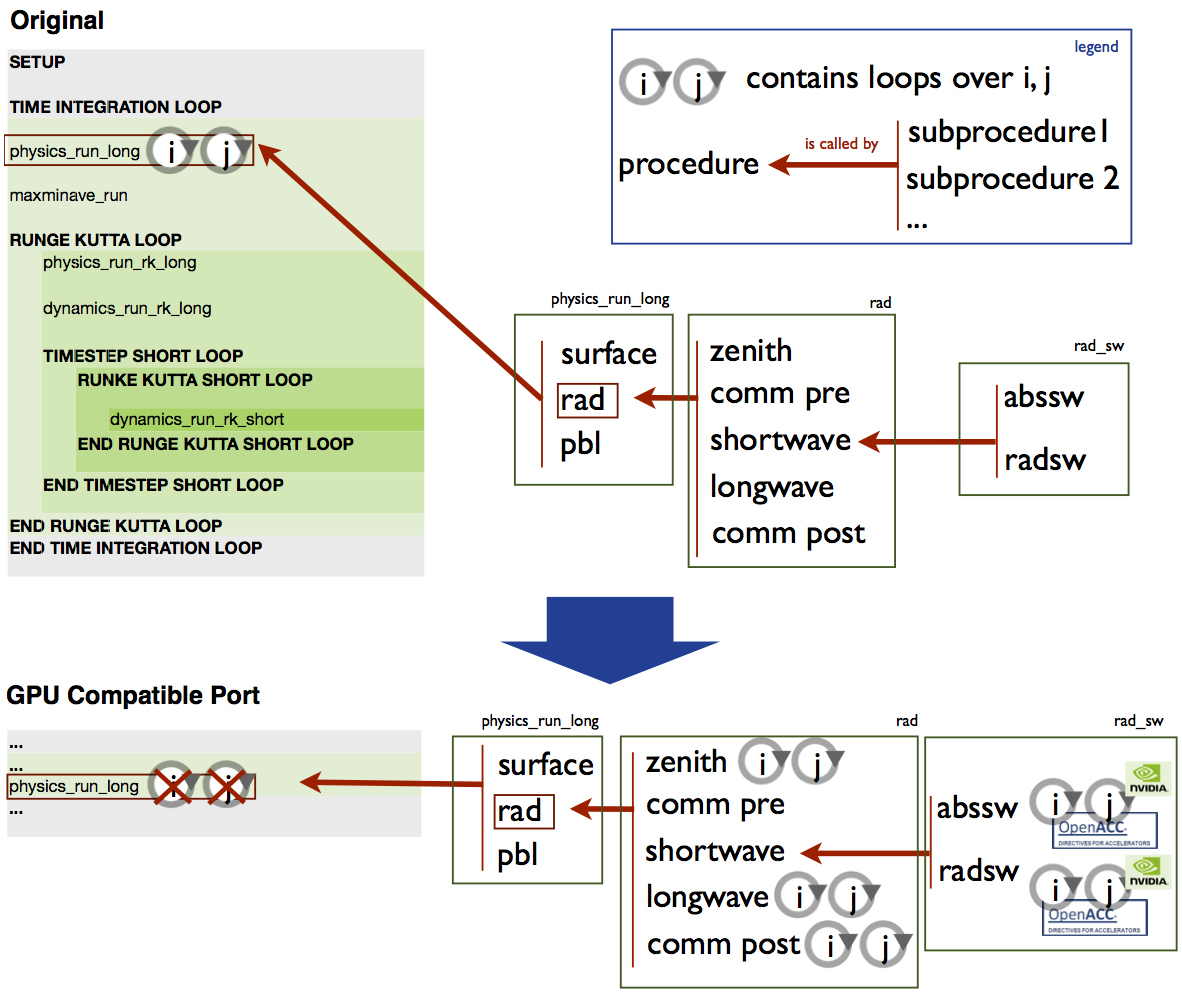
\includegraphics[width=14cm]{figures/radswOverview}
	\caption[Overview ASUCA Physical Process and Shortwave Radiation]{Overview ASUCA Physical Process and Shortwave Radiation.}
	\label{figure:overviewRadSW}
\end{figure}

Fig.~\ref{figure:overviewRadSW} depicts a reduced call graph showing only the modules concerning Shortwave Radiation and its parent callers as well as the placement of the loops. In the original code version, the loops over the \verb|I| and \verb|J| domains are placed in outside position, within the physical process interface module called by the main program loop. The data is then passed \verb|K|-column by \verb|K|-column to multiple routines, each starting a call tree. This is well suited for multicore CPU execution for two reasons: 
\begin{enumerate}
 \item For parallel execution on CPU, \textquotedblleft work packages\textquotedblright\ with long execution times (in the order of $10^{-3}\unit{s}$ or above) are preferred. The computation of one \verb|K|-column for all physical modules is fullfilling this requirement.
 \item In case of data sharing between modules, the chance for cache hits is higher if only \verb|K|-columns are being shared instead of an entire \verb|IJK|-grid of data.
\end{enumerate}

For GPUs however, this program structure is ill suited for the following reasons: 
\begin{enumerate}
 \item The number of hardware registers per kernel thread (the equivalent of a an \verb|IJ| loop run in this case) is very limited (a maximum of 63 registers are available). Having code with too much complexity inside one kernel will lead to the swapping of register data to the global memory, resulting in performance degradation in case of memory bandwidth limited programs.
 \item Kernels should ideally always operate over the same code branches. Having branches inside kernels leads to performance degradation as well, since the CUDA cores of one Warp always need to either operate over the same branch or do \verb|nop| for the diverted cycles.
 \item NVIDIA GPU architectures up until Kepler with CUDA version 5.0 (in development at the time of this thesis) do not allow native context switching for calling subroutines. Subroutine calls within kernels need to be resolved by the compiler through inlining, a process that has many limitations. As a rule of thumb, it is best to keep kernel subroutines in the same modules (source files) as the kernel and to keep only one level of subroutines below the kernel.
\end{enumerate}

Therefore, in order to create GPGPU implementations, the loops over the \verb|IJ| domains need to be implemented at a deeper call level, as shown in fig.~\ref{figure:overviewRadSW}.

\subsubsection{Execution Characteristics} \label{sub:swCharacteristics}

This module offers the following execution characteristics:
\begin{itemize}
 \item The \verb|IJ| dimensions are set to $256 \cdot 256$.
 \item The grid size in \verb|K| direction is $63$.
 \item The module is executed over one timestep.
 \item Double precision arithmetics have been used.
 \item The results have been verified using a reference CPU implementation - the root mean square deviation is in the order of $10^{-10}$.
 \item Over $95\%$ of the computational time for Shortwave radiation is being spent within the \verb|radsw| subroutine. This routine consists of approximately $300$ lines of code, executing multiple sweeps over the \verb|K| dimension for all \verb|IJ| data points and aggregating over $22$ spectra, thus containing 4th order loops. A total of $30$ \verb|ijk| data grids are accessed twice (read and write) at each data point for each of the spectra.
 \item As of expensive operations there are $22$ reciprocals being executed per data point per spectrum. NVIDIA does not specify the number of cycles needed for double precision reciprocals (they are implemented in software by the CUDA compiler). Assuming 40 cycles  per reciprocal\footnote{double the number of cycles needed by the AMD K7 CPU architecture~\cite[p. 1]{fpDivision}} this results in ${{22 \cdot 40} \over 60} \approx 14.7$ operations per fetch / write, keeping this kernel well within the memory bandwidth bounded region for the GPU. For multicore CPU we expect this module to be at the edge of being computationally bounded (since the cheap \verb|add| and \verb|mult| operations also add to the balance of the module) while for single core CPU we expect it to be clearly computationally bounded (see also sec.~\ref{sub:hardwareSystemBalance}).
 \item There are no stencil accesses with offsets in the \verb|I| or \verb|J| domain - only the \verb|K| data dimension is accessed with offsets. This is a common characteristic for all ASUCA Physical Process modules that have been examined over the course of this thesis.
\end{itemize}

Compiler flags additional to those stated in sec.~\ref{sec:investigatedFrameworks}:
\begin{description}
 \item[-Minline=levels:5,reshape] enables inlining for routines defined in the same module as their caller. The \verb|reshape| option enables the compiler to perform array reshaping when passing them to the callee.
 \item[-Mipa=inline,reshape] enables inlining for routines defined in different modules from their caller.
 \item[-r8] sets double precision as the default option for \verb|real| symbols. 
\end{description}

\clearpage
\section{Comparison of Usability} \label{sec:usabilityComparison}

In this section we compare the usability of the evaluated solutions for Fortran GPU code: CUDA Fortran, PGI OpenACC and HMPP OpenACC.

\subsection{HMPP OpenACC versus PGI OpenACC} \label{sub:hmppVsPGIUsability}

The two simple examples (particle push and 3D diffusion) have not shown major differences between HMPP OpenACC and PGI OpenACC in terms of usability. The Fortran implementation of shortwave radiation, however, has revealed some problems when using HMPP:
\begin{enumerate}
 \item Compiler errors in the tested HMPP versions often do not show line numbers, making it unnecessarily hard to find the errors in large modules.
 \item \label{enum:noScalars} HMPP implemented OpenACC kernels are not able to reference scalars, both imported from other modules and local ones, that haven't been explicitely declared with OpenACC directives or passed as arguments. 
 \item The HMPP compiler did not accept the \verb|-r8| compiler flag which tells the compiler to keep \verb|real| variables by default in double precision, a functionality that has been used within the ASUCA Physical Process.
\end{enumerate}

Especially item \ref{enum:noScalars} in the above list would have lead to major restructuring of the OpenACC code in order to ensure compatibility with HMPP. In light of the performance results shown in sec.~\ref{sec:perfEvalDiffusion} and \ref{sec:perfEvalParticle} it has been decided to not pursue this endeavor.

\subsection{Kernel Subprocedure Inlining versus Loop Restructuring} \label{sub:inliningUsability}

In sec.~\ref{sub:swDivertingGoals} a target conflict in terms of loop positionings for CPU and GPU has been introduced. Porting a CPU implementation to GPU with the parallel region loops in an outside position often leads to decisions between

\begin{itemize}
 \item trying to inline the subprocedures using compiler inlining.
 \item inlining the subprocedures manually.
 \item moving the parallel loop regions into the subprocedures, thus passing the complete data grids down to these subprocedures.
\end{itemize}

Experience has shown that inlining from other Fortran modules using Interprocedural Analysis (IPA) compiler options does not work reliably in conjunction with GPU kernel generation with \verb|pgf90| and it is best not to go that path, i.e. subprocedure calls into different modules are a clear indicator for the necessity of moving the loops into a deeper callgraph position for GPU execution. This leaves the decision for inlining within the same module. Fig.~\ref{figure:subprocUsabilityCUDA} depicts the compatibility for inlining subprocedures with CUDA while fig.~\ref{figure:subprocUsabilityOpenACC} shows the same for PGI OpenACC.

\begin{figure}[htpb]
	\centering
	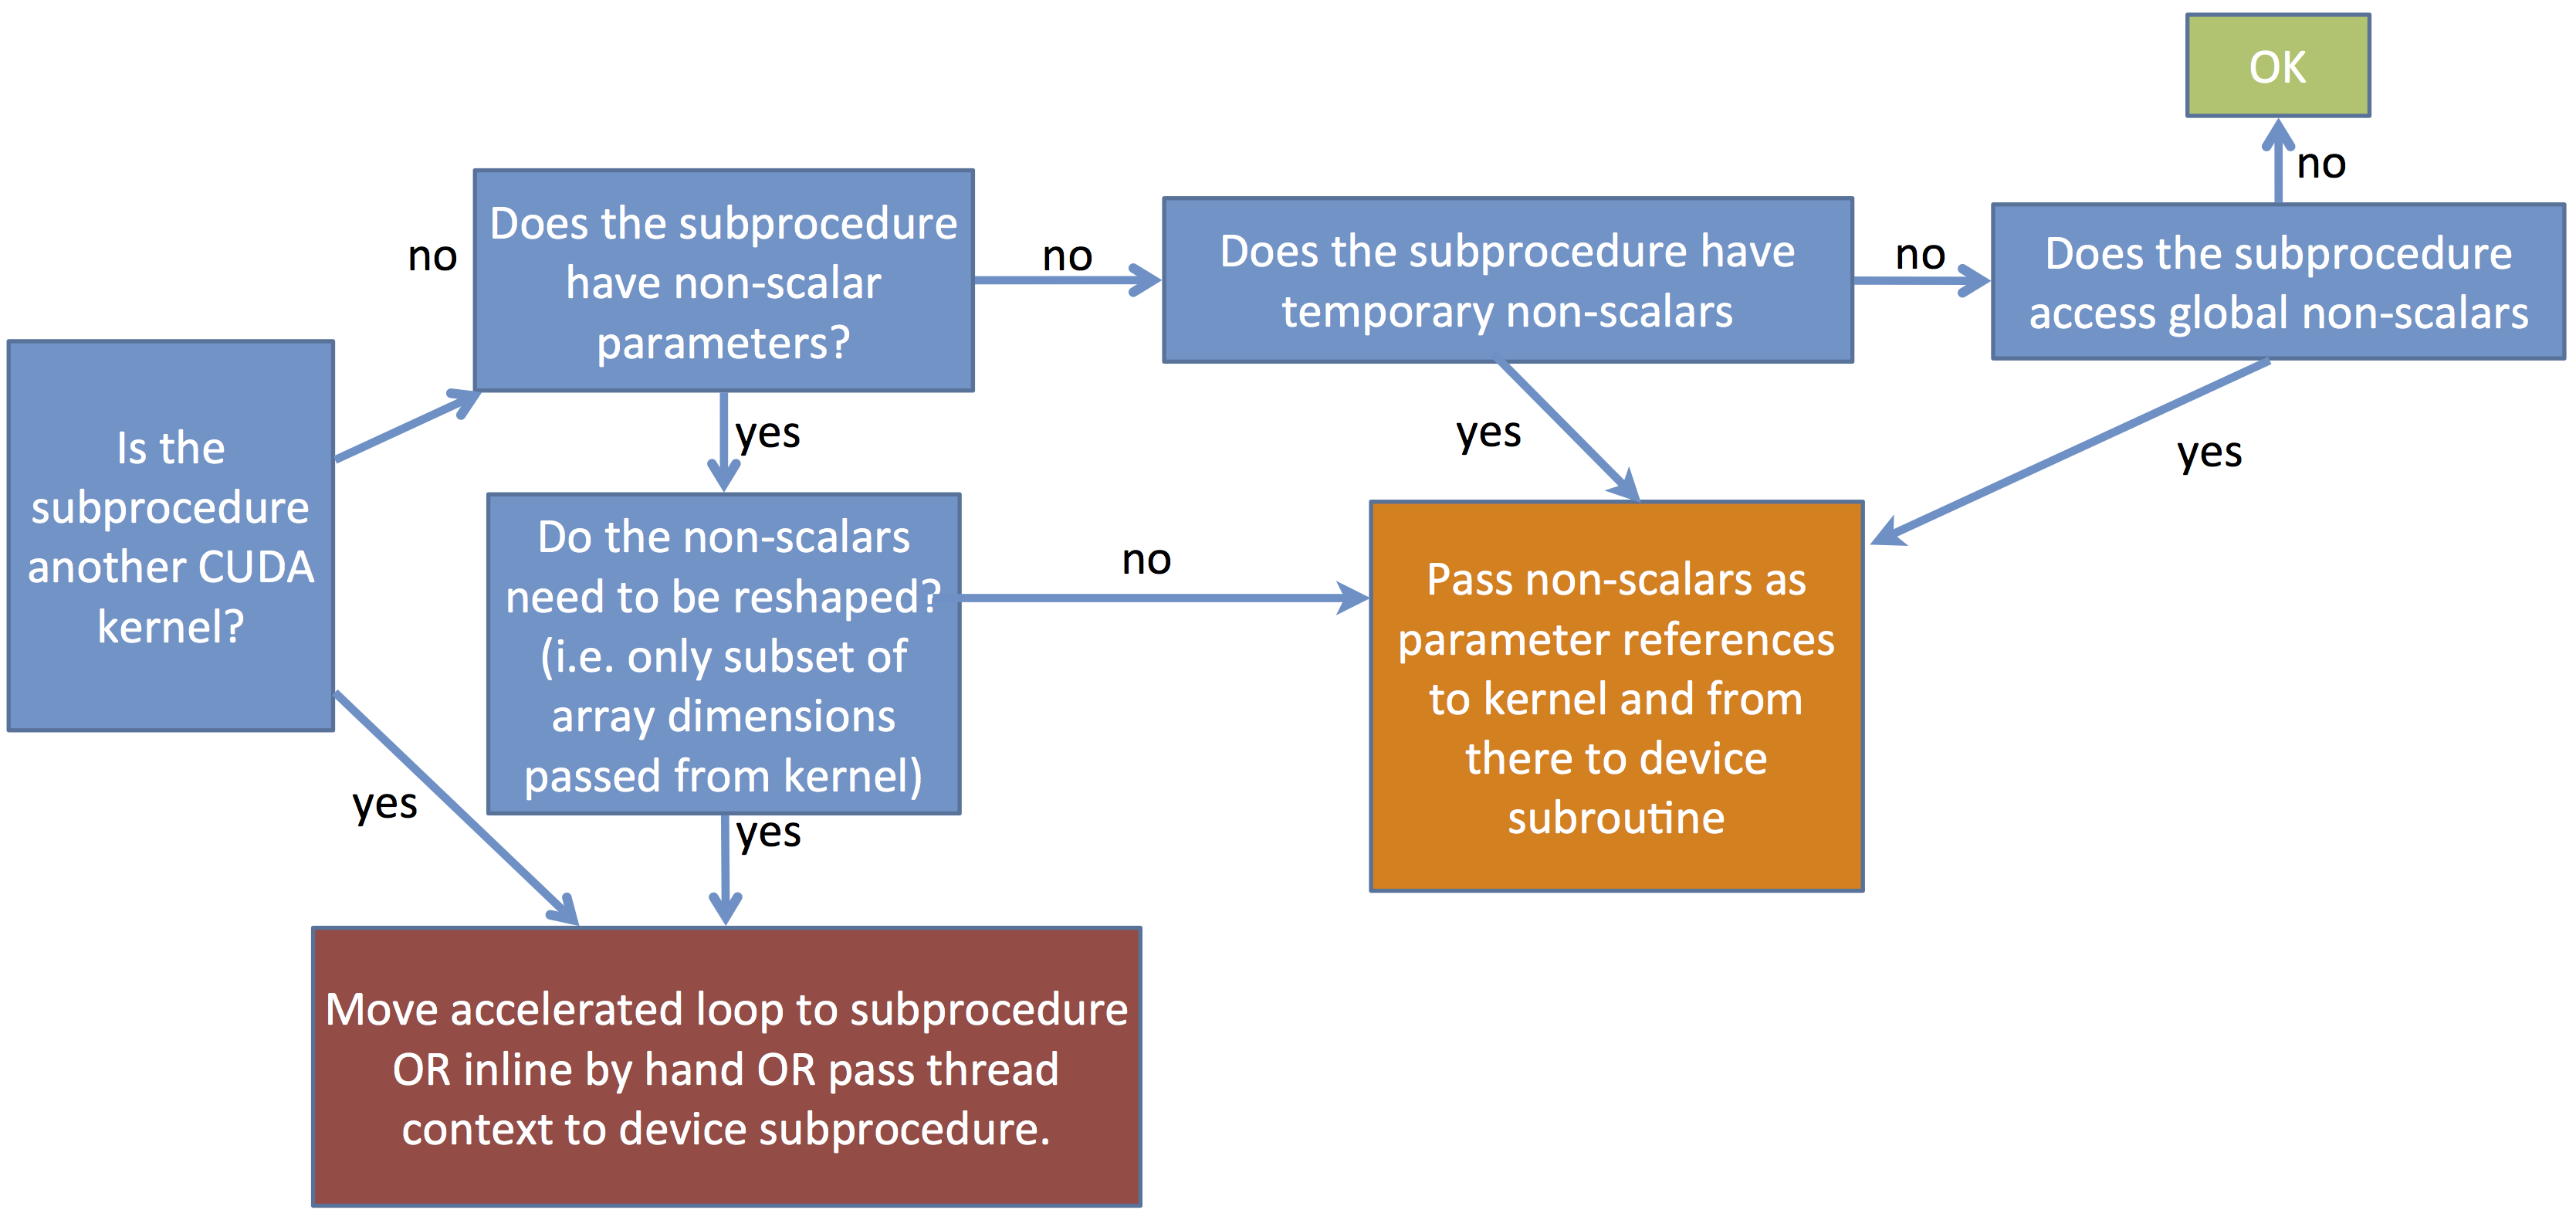
\includegraphics[width=14cm]{figures/subprocUsabilityCUDA}
	\caption[Subprocedure Inlining in CUDA Fortran]{CUDA Fortran kernel contains a device subprocedure call. Can it be inlined and therefore be compiled to device code?}
	\label{figure:subprocUsabilityCUDA}
\end{figure}

\begin{figure}[htpb]
	\centering
	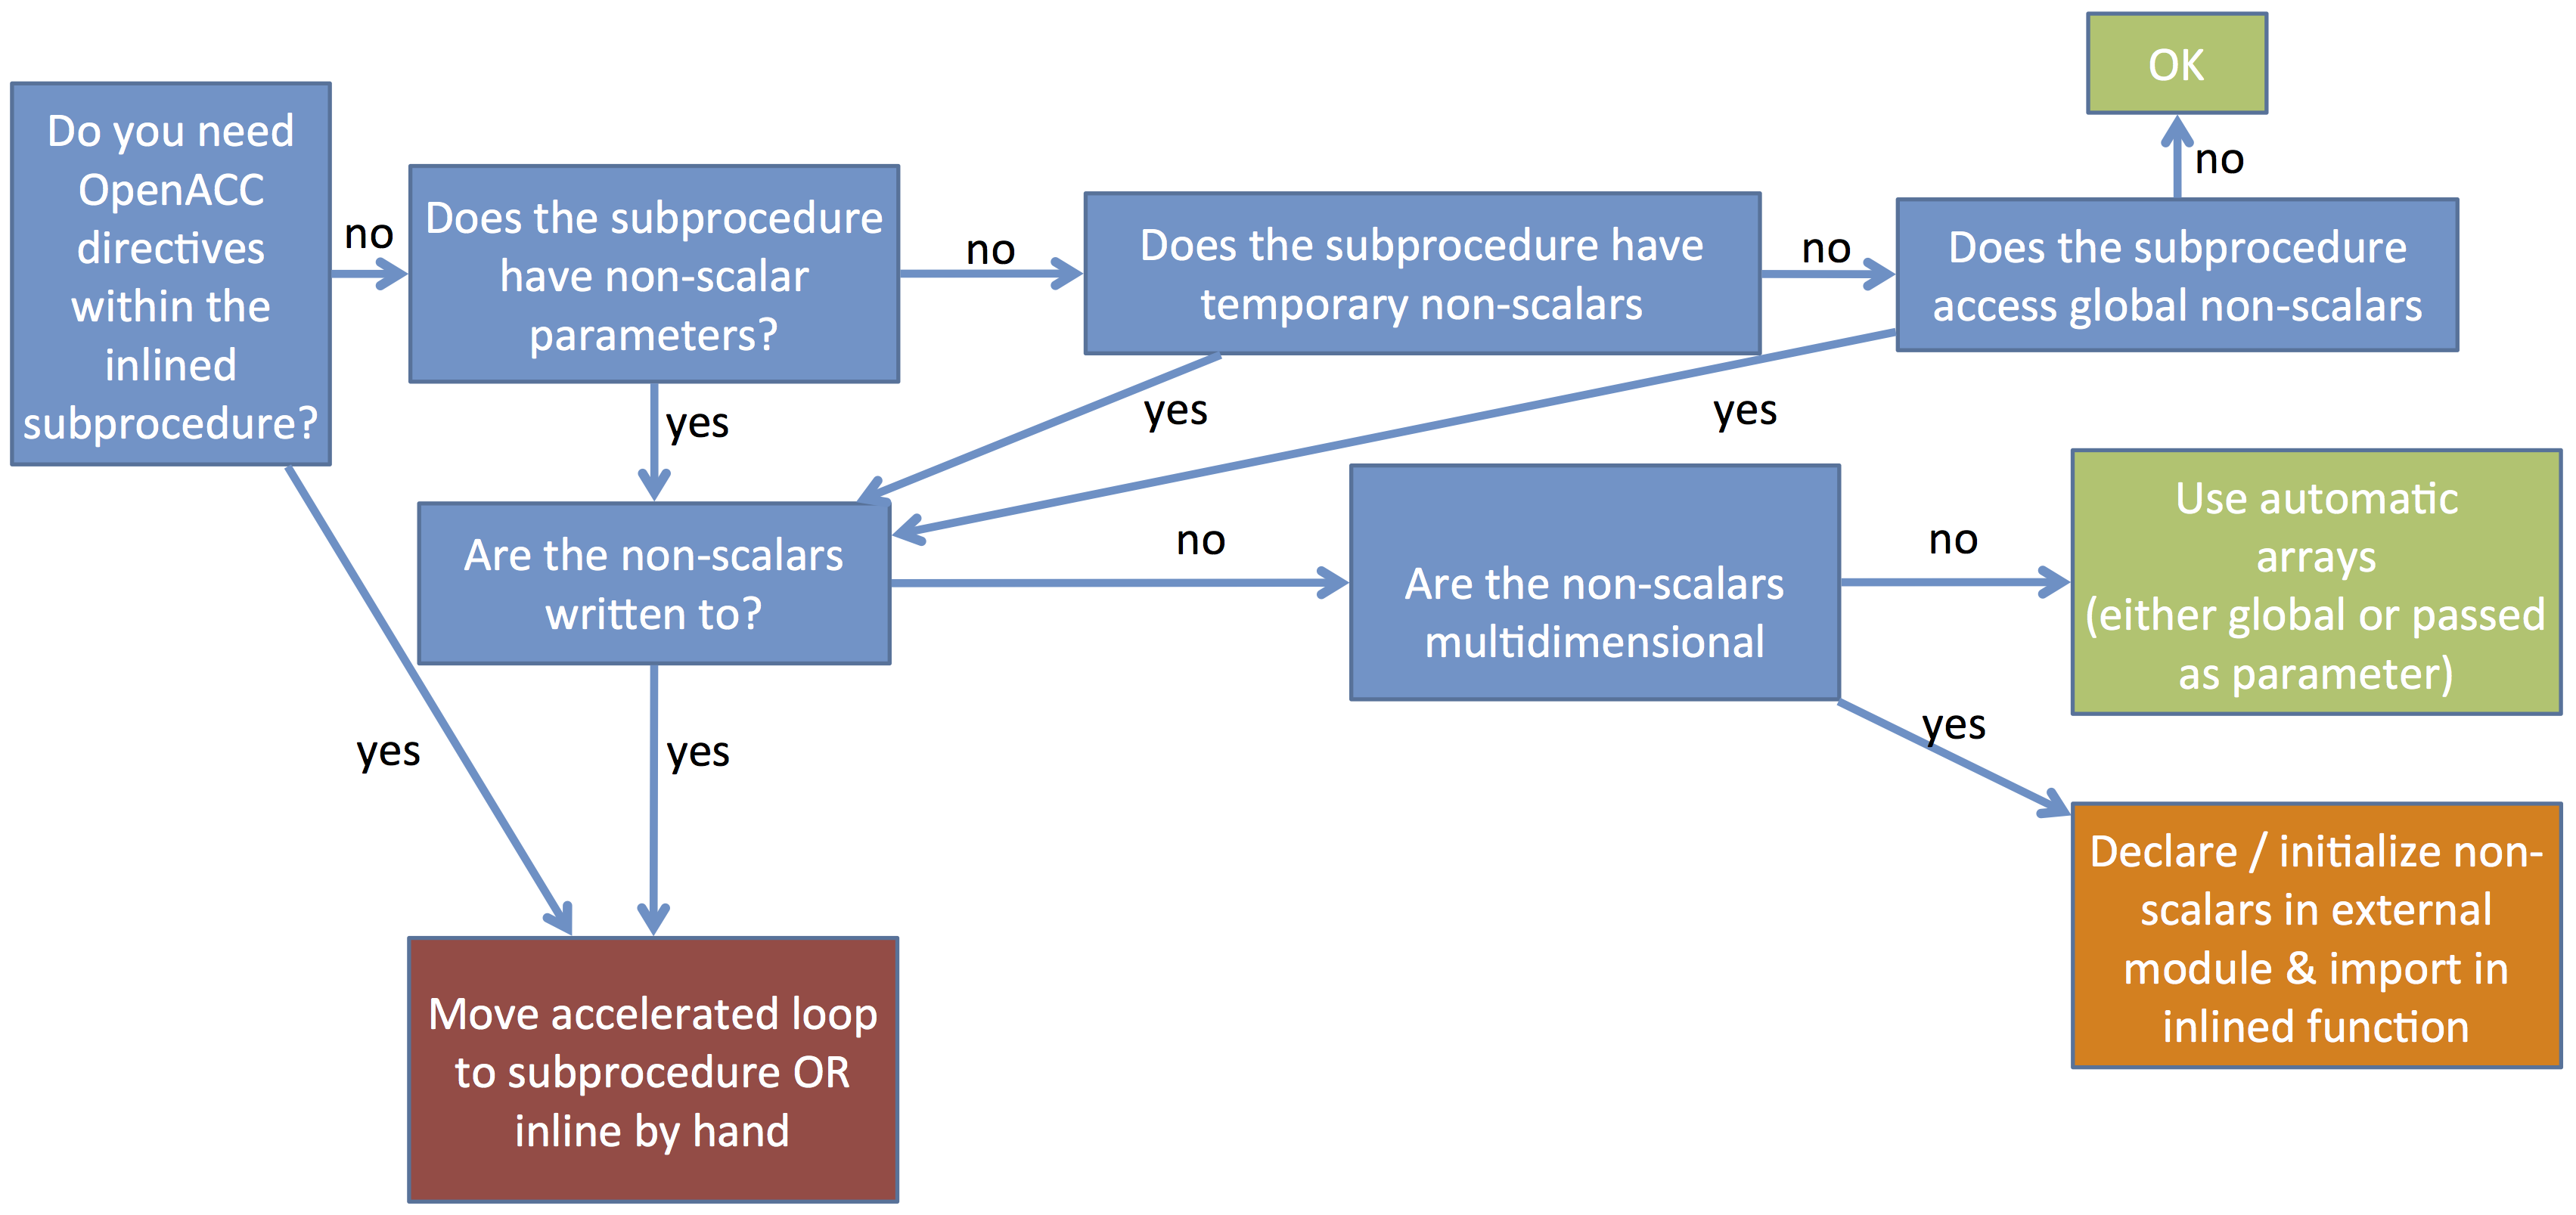
\includegraphics[width=14cm]{figures/subprocUsabilityOpenACC}
	\caption[Subprocedure Inlining in OpenACC]{PGI OpenACC accelerated region contains a subprocedure call. Can it be inlined and therefore be compiled to device code?}
	\label{figure:subprocUsabilityOpenACC}
\end{figure}

It should become clear that with these restrictions present, porting those parts of the ASUCA physical process with deep call graphs becomes a time consuming process. PGI OpenACC only offers limited help in that regard. Its advantages in comparison to CUDA Fortran in terms of porting code of the nature of the ASUCA physical process, are as follows: 
\begin{enumerate}
 \item \label{enum:multiLoops} The ability to introduce multiple parallel loops within one subprocedure.
 \item \label{enum:oneDimModuleArray} The ability to use one dimensional module arrays.
 \item \label{enum:localArray} The ability to use local arrays within kernel subroutines (not within device subroutines called by kernels however).
\end{enumerate}

Item \ref{enum:multiLoops} saves the introduction of some subprocedures, however one could argue that the splitting of code into multiple subprocedures may in that case lead to a clearer, more maintainable codebase. Items \ref{enum:oneDimModuleArray} and \ref{enum:localArray} allow the use of preinitialised data and local arrays without passing them as parameters to kernels. However experience has shown that the most significant portation cost lays in the restructuring of data accesses, data parameters and loops to meet the requirements of GPU execution - an area in which OpenACC does not offer an advantage over CUDA Fortran.


\subsection{Overview Usability} \label{sub:overviewUsability}

Tab.~\ref{table:usabilityFortranGPU} gives an overview over the usability issues we have found when porting CPU code to the GPU using one of the aforementioned frameworks.

\begin{savenotes}\begin{table}[htpb]
	\centering
	\footnotesize
	\begin{tabular}{l|c|c|c}
		Issue & CUDA Fortran & PGI OpenACC & HMPP OpenACC \\ 
		\hline \hline
		Subprocedure calls in & see figure \ref{figure:subprocUsabilityCUDA} & see figure \ref{figure:subprocUsabilityOpenACC} & Not examined \\
		parallel regions possible & & & \\
		\hline
		Subprocedure calls from & No & No & Not examined \\
		different modules possible & & & \\
		\hline
		Multiple parallel regions & No & Yes & Yes \\
		per subroutine & & \\
		\hline
		Automatic device data copies & No & Yes & Yes \\
		\hline
		Use of local scalars & Yes & Yes & Needs directives \\
		\hline
		Use of local arrays & No & Yes & Not examined \\
		\hline
		Use of scalars imported & No & Yes & No \\
		from external modules & & & \\
		\hline
		Recursive subprocedures & No & No & No \\
		\hline
		Inline array initialisations & No & No & No \\
		\hline
		\verb|SAVE|, \verb|DATA| attributes & No & No & No \\
		\hline
		Abstraction of parallel & No & No & No \\
		domain dependency & & & \\
		\hline
	\end{tabular}
	\caption[Usability Issues GPGPU in Fortran]{Usability issues with GPGPU in Fortran.}
	\label{table:usabilityFortranGPU}
\end{table}\end{savenotes}


\clearpage
\section{Comparison of Performance} \label{sec:perfEvaluation}

In this section the performance comparisons between CPU execution, OpenACC GPU execution and CUDA will be discussed.

\subsection{Overview of Tests}

The following table gives an overview over the preliminarily investigated GPGPU technologies and the applied test cases.

\begin{table}[htpb]
	\centering
	\footnotesize
	\begin{tabular}{l|c|c|c}
		Framework & Version & Maintainer & Test Cases \\ 
		\hline \hline
		PGI OpenACC & 12.4 & PGI & Particle Push,\\ 
		For C Language & & & 3D Diffusion \\
		\hline
		PGI OpenACC & 12.4 & PGI & ASUCA Shortwave Radiation \\ 
		For Fortran Language & & & \\
		\hline
		HMPP OpenACC & 3.1.0 & CAPS & Particle Push,\\
		For C Language & & & 3D Diffusion \\
		\hline
		HMPP OpenACC & 3.1.0 & CAPS & None, see sec.~\ref{sub:hmppVsPGIUsability}\\
		For Fortran Language & & & \\
		\hline
		CUDA C & 4.1 & NVIDIA & Particle Push,\\
		& & & 3D Diffusion \\
		\hline
		CUDA Fortran & 12.4 & PGI & ASUCA Shortwave Radiation \\ 
		\hline
	\end{tabular}
	\caption[Overview Framework Tests]{Overview frameworks and test cases.}
	\label{table:testsByFrameworksOverview}
\end{table}

For the test platform's hardware specifications please refer to sec.~\ref{sec:testHardware}. 

All results shown here have been averaged over 5 runs. Only computation time, no host-to-device data copy time has been counted, since the host-to-device bus performance is not expected to be relevant for ASUCA (the goal is a complete GPU portation, making data copying only necessary at the beginning and end of the simulation, thus significantly reducing communication overhead). 

\subsection{3D Diffusion} \label{sec:perfEvalDiffusion}

Fig.~\ref{figure:diffusionExecTime} and fig.~\ref{figure:diffusionSpeedup} illustrate the following examinations: 

\begin{enumerate}
 \item The magnitude of speedups further indicate that this algorithm is being bounded by memory bandwidth (as estimated in sec.~\ref{sub:test3DDiffusion}).
 \item The speedups of GPU implementations versus the CPU implementation are in line with the hardware model introduced in sec.~\ref{sub:hardwarePerfOverview} for the single precision results. The double precision speedup is lower than expected however (speedups of the same magnitude as single precision execution are expected for double precision execution). Considering the execution time results shown in fig.~\ref{figure:diffusionExecTime} the CUDA and PGI OpenACC implementations scale as expected (around a factor of two), however CPU execution as well as HMPP do not scale as expected, indicating some overhead being present in their single precision versions. Considering, that this algorithm is most likely heavily bounded by memory bandwidth, overfetches are a likely candidate for the deviations from the model - i.e. data is being read into cache that is not needed by the active thread - a phenomenon that is less strong with double precision execution, since the payload data is always twice the size. It is 
therefore likely that this 
algorithm could be further optimized by optimizing the code for cache accesses - however this kind of optimization is very specific to the architecture. 
 \item PGI OpenACC performs significantly better than HMPP for this example. 
 \item CUDA Fortran performs significantly better than the OpenACC implementations in the single precision case. In double precision, CUDA Fortran and PGI Fortran perform very similarly.
\end{enumerate}

\begin{figure}[htpb]
	\centering
	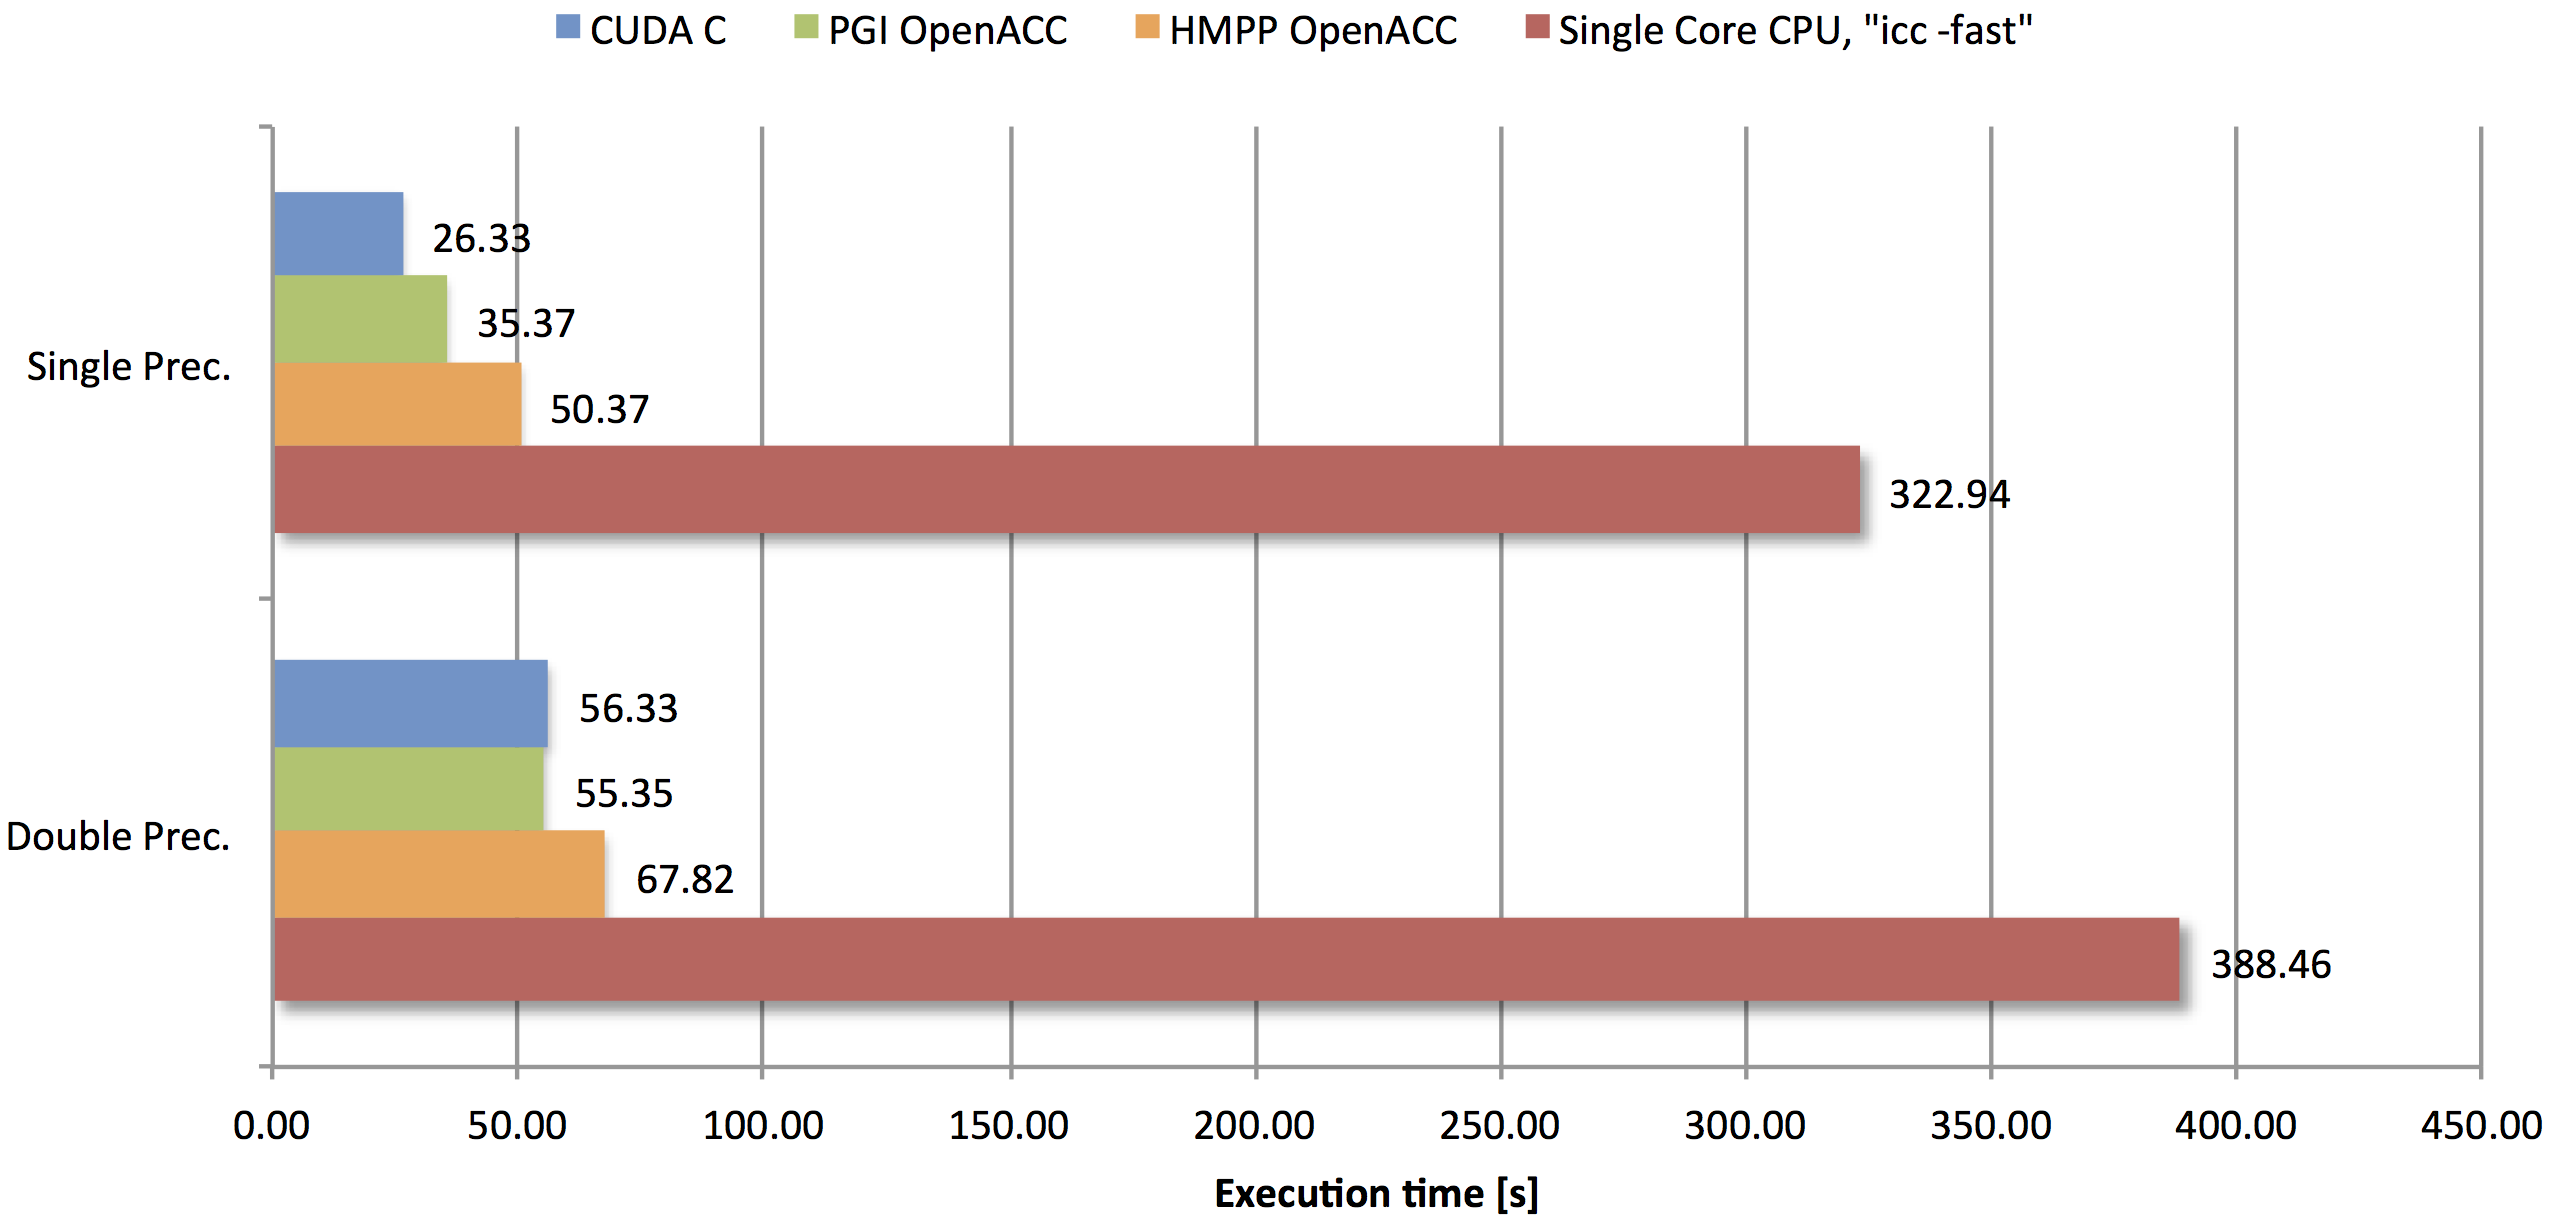
\includegraphics[width=14cm]{figures/diffusionExecTimeResults}
	\caption[Execution Time Results for 3D Diffusion]{Execution time results for the 3D Diffusion Algorithm.}
	\label{figure:diffusionExecTime}
\end{figure}

\begin{figure}[htpb]
	\centering
	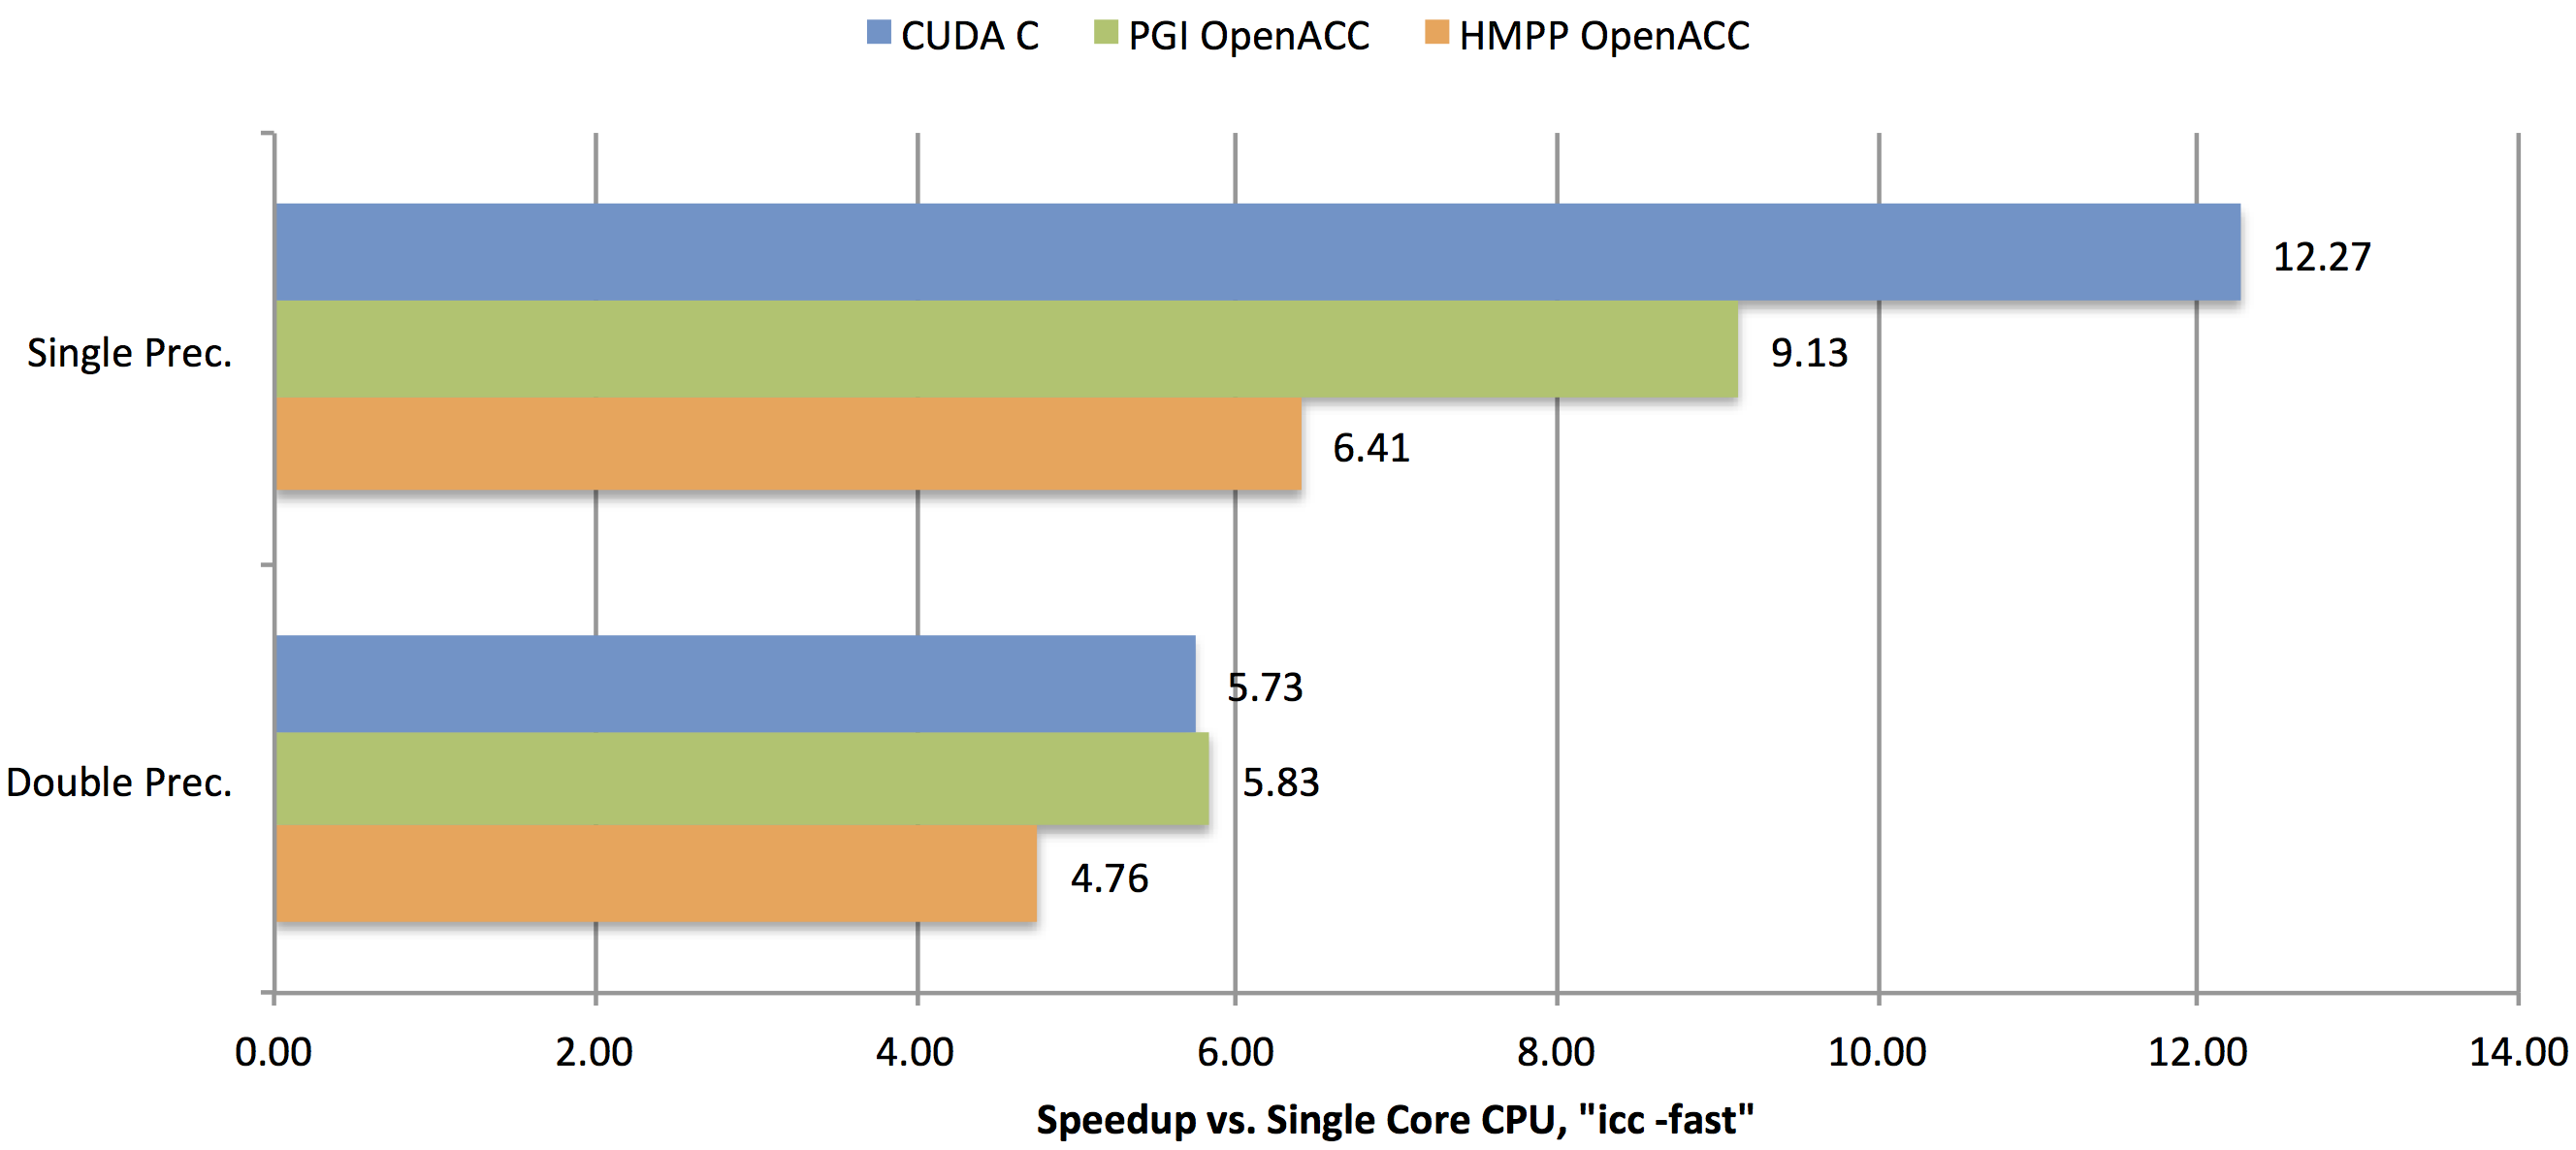
\includegraphics[width=14cm]{figures/diffusionSpeedupResults}
	\caption[Speedup Results for 3D Diffusion]{Speedup results for the 3D Diffusion Algorithm when compared to Single Core CPU, ``icc -fast'' compiled.}
	\label{figure:diffusionSpeedup}
\end{figure}

\clearpage
\subsection{Particle Push} \label{sec:perfEvalParticle}

\begin{figure}[htpb]
        \centering
        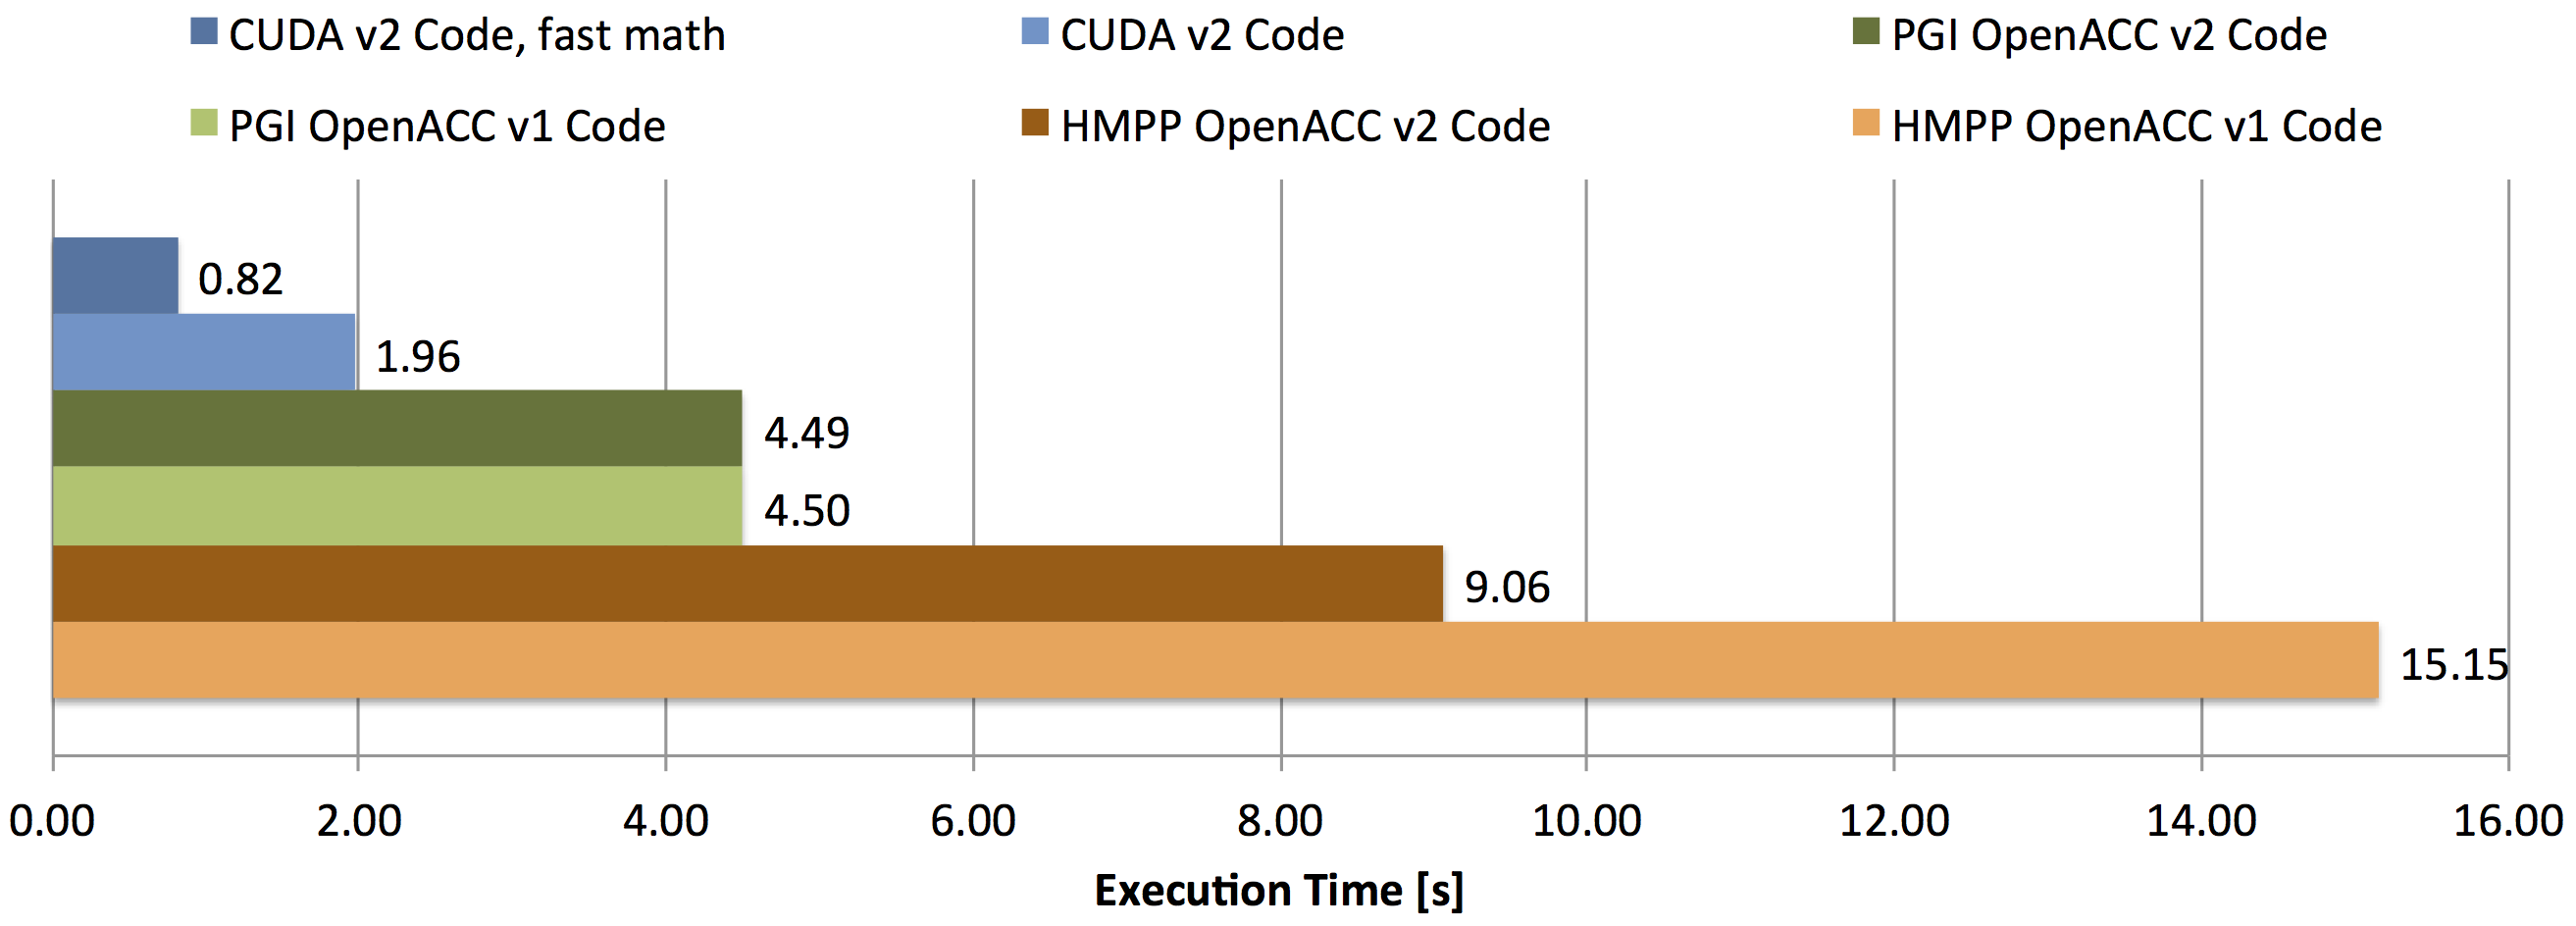
\includegraphics[width=14cm]{figures/particleExecTimeResults}
        \caption[Execution Time Results for Particle Push]{Single precision execution time results for the Particle Push Algorithm. CPU results are not shown here since the two orders of magnitude difference would make it hard to distinguish the GPU results.}
        \label{figure:particleExecTime}
\end{figure}

\begin{figure}[htpb]
        \centering
        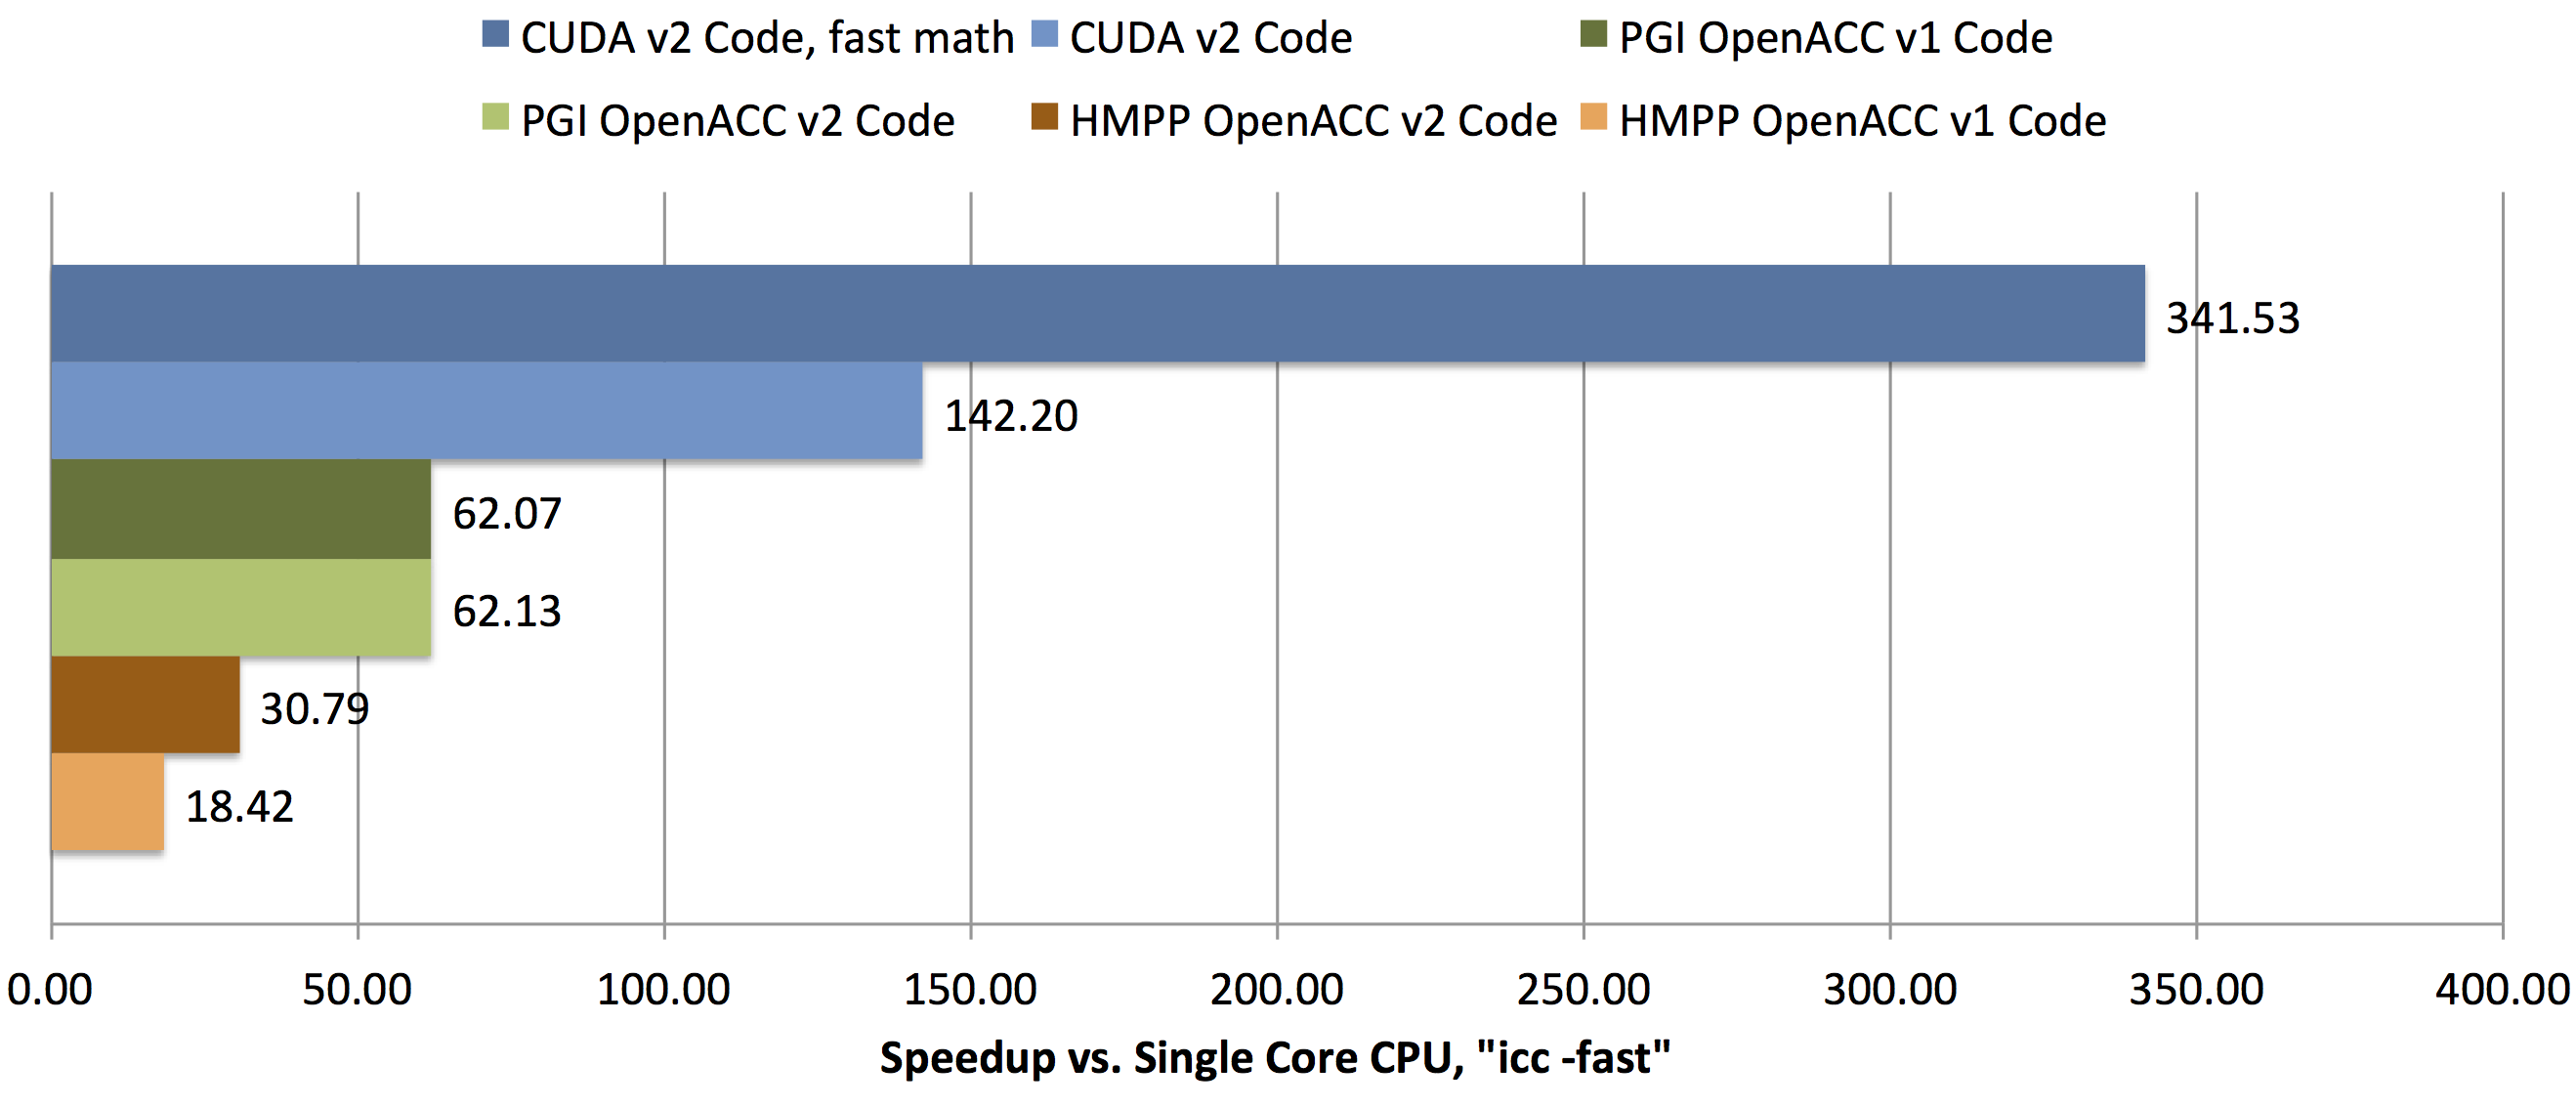
\includegraphics[width=14cm]{figures/particleSpeedupResults}
        \caption[Speedup Results for Particle Push]{Single precision speedup results for the Particle Push Algorithm when compared to Single Core CPU, ``icc -fast'' compiled, v1 Code.}
        \label{figure:particleSpeedup}
\end{figure}

Fig.~\ref{figure:particleExecTime} and fig.~\ref{figure:particleSpeedup} illustrate the following examinations: 

\begin{enumerate}
 \item The speedups of GPU implementations versus the CPU implementation observed with this example are significantly higher than what one could expect from the performance metrics assessed in sec.~\ref{sec:testHardware}. This indicates the following: 
 \begin{enumerate}
  \item This algorithm is indeed computationally bounded as assumed in sec.~\ref{sub:testParticlePush}. Speedups of this magnitude for memory bandwidth bounded problems are highly unlikely. 
  \item The provided GPU architecture as well as the CUDA compiler appear to be more optimized for Sine- and Cosine operations. This is a reasonable assumption to make since Sine- and Cosine operations are very important for geometrical computations, one of the key areas of the GPU. 
  \item It is likely that the CPU implementation could still be optimized by a significant margin.
 \end{enumerate}
 \item PGI OpenACC performs significantly better than HMPP for this example.
 \item PGI OpenACC doesn't show a significant improvement between the code versions 1 and 2 (see sec.~\ref{sub:testParticlePush}). An examination of the CUDA C code created by the PGI OpenACC compiler has revealed that the PGI compiler is able to perform these optimizations for the code version 1 as well.
 \item The CUDA version is still faster by a factor of $2.3$ compared to the PGI OpenACC code. The code examination of PGI OpenACC's created code has revealed that there are additional safety branches being added to the kernel code - which is not needed for the CUDA code implemented by hand, since the programmer is able to configure the kernel in a way that it will not exceed the data boundaries. One would expect this to be the reason for the slowdown of the PGI OpenACC version. 
 \item The \verb|fastmath| special function units (a hardware implementation of Sine- and Cosine functions among others) are not responsible for the above mentioned speedup of CUDA vs. OpenACC, since enabling \verb|fastmath| gives an additional speedup factor of $2.4$. Note: Doing so results in a slight loss in fidelity (the GPU's root mean square error versus reference result changes from $1.62 \cdot 10^{-6}$ to $2.33 \cdot 10^{-6}$).
\end{enumerate}

\clearpage
\subsection{ASUCA Shortwave Radiation} \label{perfEvalShortwave}

This section shows the performance test results for the ASUCA shortwave radiation module. Since OpenACC allows hybrid execution, it was also tested how a hybridized CUDA version compares in terms of CPU performance. Therefore the CUDA Fortran version has been implemented using preprocessor directives in order to hybridize that codebase\footnote{E.g. the CUDA kernels have been wrapped in ``do''/``end do'' loops over the ``IJ'' domain for CPU execution.}, rendering the kernel code compatible for CPU execution after the preprocessor.  This hybridized CUDA version will be referred to as \textquotedblleft Preprocessed CUDA Fortran\textquotedblright. Some performance loss on the CPU was expected since the loop structure for these implementations is optimized for GPU execution (see also sec.~\ref{sub:swDivertingGoals}).

Fig.~\ref{figure:radswExecTime} and fig.~\ref{figure:radswSpeedup} illustrate the following: 

\begin{enumerate}
 \item The magnitude of speedups further indicate that this algorithm is being bounded by memory bandwidth (as estimated in sec.~\ref{sub:testASUCARadSW} for GPU execution).
 \item The speedups of GPU implementations versus the CPU implementation are only slightly below what is expected for memory bandwidth limited modules as outlined in sec.~\ref{sub:hardwarePerfOverview}. Judging from the hardware model another 10\% speedup could be expected from further optimizing the GPU version.
 \item The GPU results of PGI OpenACC are only approximately 5\% below those of CUDA Fortran. This indicates that the advantage of CUDA Fortran vs. OpenACC shrinks for larger kernels, when the additions of safety branches (as discussed in sec.~\ref{sec:perfEvalParticle}) are not as significant anymore compared to the overall load.
 \item Executing code with loops optimized for GPU execution on the CPU results in a $2\times$ performance loss in this case. The preprocessed CUDA Fortran code handles this slightly worse than the PGI OpenACC version, loosing another 15\%.
\end{enumerate}

\begin{figure}[htpb]
	\centering
	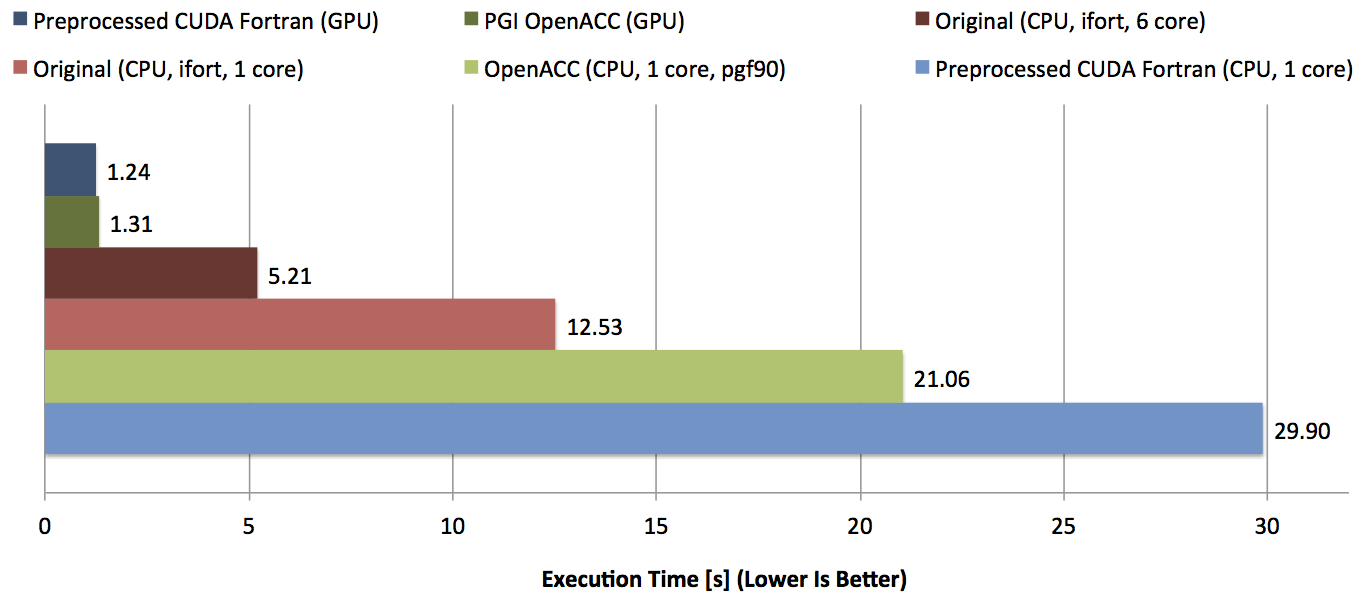
\includegraphics[width=14cm]{figures/radswExecTimeResults}
	\caption[Execution Time Results for Shortwave Radiation]{Double precision execution time results for the shortwave radiation module.}
	\label{figure:radswExecTime}
\end{figure}

\begin{figure}[htpb]
	\centering
	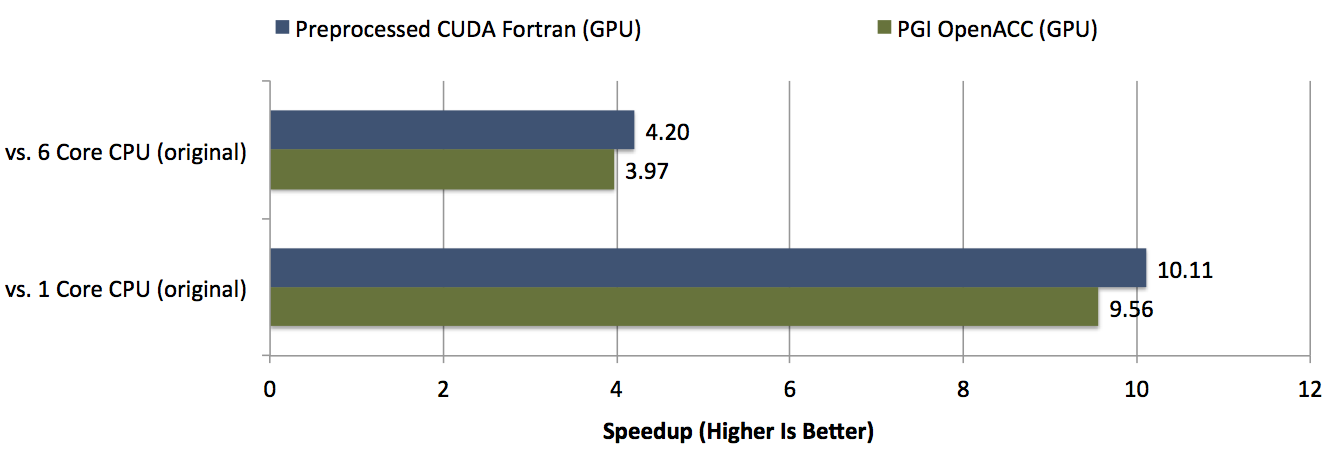
\includegraphics[width=14cm]{figures/radswSpeedup}
	\caption[Speedup Results for Shortwave Radiation]{Double precision speedup results for the shortwave radiation module when compared to CPU execution of the original code version, ``icc -fast'' compiled.}
	\label{figure:radswSpeedup}
\end{figure}

\clearpage
\section{Preliminary Conclusions} \label{sec:evalConclusion}

I would like to draw the following preliminary conclusions regarding the results from sec.~\ref{sec:usabilityComparison} and sec.~\ref{sec:perfEvaluation}: 

\begin{enumerate}
 \item \label{enum:targetConflict} Porting code with complex call graphs inside parallel regions to GPU will result in the following target conflict:
  \begin{enumerate}
    \item Optimization for GPU results in low performance on the CPU. Fig.~\ref{figure:radswExecTime} illustrates this point conclusively.
    \item Optimization for CPU lowers GPU performance and even breaks GPU compatibility at some point.
  \end{enumerate}
 \item \label{enum:portationCost} Changing the loop structure and data accesses is considered to be the most time consuming task for porting the ASUCA physical process to GPU.
 \item In case the OpenACC route is to be pursued, the results shown in this thesis indicate a clear advantage of PGI over HMPP, both in usability and performance. Please note, however, that OpenACC support has still been under heavy development during the timeframe of this thesis - later versions would have to be reexamined.
 \item PGI OpenACC is able to perform rather intricate optimizations of arithmetics, as shown in sec.~\ref{sec:perfEvalParticle}. Kernel code created by PGI OpenACC might be helpful to examine in case of computationally bounded code.
 \item The speedup estimates for the three test examples based on the hardware model introduced in sec.~\ref{sec:testHardware} have proven to be reasonable and may be taken into consideration for further analysis.
\end{enumerate}

Items \ref{enum:targetConflict} and \ref{enum:portationCost} in the above list lead to the following question: Is there a solution offering
\begin{enumerate}
 \item lower portation cost than OpenACC,
 \item high GPU performance and
 \item high CPU performance?
\end{enumerate}

The following chapters will answer this question.